\documentclass[article]{uom-coursework}
\usepackage[showframe]{geometry}

\usetikzlibrary{automata, positioning, arrows,
arrows.meta}

\usepackage{float}
\usepackage{syntax}
\usepackage{mdframed}
\usepackage[ruled]{algorithm2e}
\usepackage[nopagecolor={white}]{pagecolor}
% \usepackage{contour}
\usepackage{soul}
\usepackage{calc}
% \usepackage{svg}
% \usepackage{wrapfig2}
\usepackage{bytefield}
\usepackage{adjustbox}
% \usepackage[normalem]{ulem}
% \usepackage[luatex]{accsupp}

\usepackage{caption}
\usepackage{subcaption}

\newcommand{\legendbox}[1]{%
\textcolor{#1}{\rule{\fontcharht\font`X}{\fontcharht\font`X}}%
}

\definecolor{pastelblue}{HTML}{aec6cf}
\definecolor{pastelpink}{HTML}{ffd1dc}
\definecolor{pastelgreen}{HTML}{b0e57c}
\definecolor{pastelgrey}{HTML}{d3d3d3}

% \setlength{\ULdepth}{1.8pt}
% \contourlength{1pt}

% \newcommand{\ul}[1]{
% \BeginAccSupp{method=plain,ActualText={#1}}%
% \uline{\hphantom{#1}}%
% % \llap{\contour{\thepagecolor}{#1}}%
% \EndAccSupp{}%
% }

% \newcommand{\ul}[1]{
% \uline{\hphantom{#1}}%
% \llap{#1}%
% }

\usepackage{caption}
\captionsetup{%
   % labelsep=newline,
   justification=raggedright,
   labelfont=bf
}

\tcbuselibrary{most,documentation}

\tcbset{skin=enhanced,
  doc head={colback=yellow!10!white,interior style=fill},
  doc head key={colback=magenta!5!white,interior style=fill},
  doc head path={colback=blue!50!gray!7!white,interior style=fill},
  color key=DarkViolet,
  color value=Teal,
  color color=Teal,
  color counter=Orange!85!black,
  color length=Orange!85!black,
  index colorize,
  index annotate,
}

\newtcolorbox{marker}[1][]{
  before skip balanced=2mm,after skip balanced=3mm,
  boxrule=0.4pt,left=5mm,right=2mm,top=1mm,bottom=1mm,
  colback=UMc2!50,
  colframe=UMc2!20!black,
  sharp corners,rounded corners=southeast,arc is angular,arc=3mm,
  underlay={%
    \path[fill=tcbcolback!80!black] ([yshift=3mm]interior.south east)--++(-0.4,-0.1)--++(0.1,-0.2);
    \path[draw=tcbcolframe,shorten <=-0.05mm,shorten >=-0.05mm] ([yshift=3mm]interior.south east)--++(-0.4,-0.1)--++(0.1,-0.2);
    \path[fill=UMc2!50!black,draw=none] (interior.south west) rectangle node[white]{\Huge\bfseries !} ([xshift=4mm]interior.north west);
    },
  drop fuzzy shadow,#1}

\newlength\inlineheight
\newlength\inlinedepth
\settototalheight\inlineheight{Xygp}
\settodepth\inlinedepth{Xygp}
\setlength\fboxsep{0pt}
\newcommand*\inlinegraphics[1]{%
  \settototalheight\inlineheight{Xygp}%
  \settodepth\inlinedepth{Xygp}%
  \raisebox{-\inlinedepth}{\includegraphics[height=\inlineheight]{#1}}%
}



\newtcolorbox{todo}[1][]{
  before skip balanced=2mm,after skip balanced=3mm,
  boxrule=0.4pt,left=5mm,right=2mm,top=1mm,bottom=1mm,
  colback=UMc17!50,
  colframe=UMc17!20!black,
  sharp corners,rounded corners=southeast,arc is angular,arc=3mm,
  underlay={%
    \path[fill=tcbcolback!80!black] ([yshift=3mm]interior.south east)--++(-0.4,-0.1)--++(0.1,-0.2);
    \path[draw=tcbcolframe,shorten <=-0.05mm,shorten >=-0.05mm] ([yshift=3mm]interior.south east)--++(-0.4,-0.1)--++(0.1,-0.2);
    \path[fill=UMc17!50!black,draw=none] (interior.south west) rectangle node[white]{\rotatebox{90}{\resizebox{!}{0.6em}{\bfseries TODO}}} ([xshift=4mm]interior.north west);
    },
  drop fuzzy shadow,#1}

\newtcolorbox{note}[1][]{
  before skip balanced=2mm,after skip balanced=3mm,
  boxrule=0.4pt,left=5mm,right=2mm,top=1mm,bottom=1mm,
  colback=UMc8!50,
  colframe=UMc8!20!black,
  sharp corners,rounded corners=southeast,arc is angular,arc=3mm,
  underlay={%
    \path[fill=tcbcolback!80!black] ([yshift=3mm]interior.south east)--++(-0.4,-0.1)--++(0.1,-0.2);
    \path[draw=tcbcolframe,shorten <=-0.05mm,shorten >=-0.05mm] ([yshift=3mm]interior.south east)--++(-0.4,-0.1)--++(0.1,-0.2);
    \path[fill=UMc8!50!black,draw=none] (interior.south west) rectangle node[white]{\rotatebox{90}{\resizebox{!}{0.6em}{\bfseries NOTE}}} ([xshift=4mm]interior.north west);
    },
  drop fuzzy shadow,#1}


\newtcolorbox{noteline}[1][]{
  before skip balanced=2mm,after skip balanced=3mm,
  boxrule=0.4pt,left=5mm,right=2mm,top=1mm,bottom=1mm,
  colback=UMc8!50,
  colframe=UMc8!20!black,
  sharp corners,rounded corners=southeast,arc is angular,arc=3mm,
  underlay={%
    \path[fill=tcbcolback!80!black] ([yshift=3mm]interior.south east)--++(-0.4,-0.1)--++(0.1,-0.2);
    \path[draw=tcbcolframe,shorten <=-0.05mm,shorten >=-0.05mm] ([yshift=3mm]interior.south east)--++(-0.4,-0.1)--++(0.1,-0.2);
    \path[fill=UMc8!50!black,draw=none] (interior.south west) rectangle node[white]{\rotatebox{90}{\resizebox{!}{0.4em}{\bfseries NOTE}}} ([xshift=4mm]interior.north west);
    },
  drop fuzzy shadow,#1}

\newtcolorbox{attrib}[1][]{
  before skip balanced=2mm,after skip balanced=3mm,
  boxrule=0.4pt,left=5mm,right=2mm,top=1mm,bottom=1mm,
  colback=UMc16!50,
  colframe=UMc16!20!black,
  sharp corners,rounded corners=southeast,arc is angular,arc=3mm,
  underlay={%
    \path[fill=tcbcolback!80!black] ([yshift=3mm]interior.south east)--++(-0.4,-0.1)--++(0.1,-0.2);
    \path[draw=tcbcolframe,shorten <=-0.05mm,shorten >=-0.05mm] ([yshift=3mm]interior.south east)--++(-0.4,-0.1)--++(0.1,-0.2);
    \path[fill=UMc16!50!black,draw=none] (interior.south west) rectangle node[white]{\rotatebox{90}{\resizebox{!}{0.5em}{\bfseries ATTRIB.}}} ([xshift=4mm]interior.north west);
    },
  drop fuzzy shadow,#1}

\newtcolorbox{framefig}{
    boxrule=1pt,
    boxsep=0pt,
    sharp corners,
    colback=white,
    left=0pt,
    right=0pt,
    top=0pt,
    bottom=0pt
}

\definecolor{UMPaleRed}{HTML}{d29599}
\definecolor{OffWhite}{HTML}{fffff4}

\makeatletter
\newcommand{\RemoveAlgoNumber}{\renewcommand{\fnum@algocf}{\AlCapSty{\AlCapFnt\algorithmcfname}}}
\newcommand{\RevertAlgoNumber}{\algocf@resetfnum}
\makeatother

% \usepackage{etoolbox}% http://ctan.org/pkg/etoolbox
% \makeatletter
% \patchcmd{\lst@GLI@}% <command>
%   {\def\lst@firstline{#1\relax}}% <search>
%   {\def\lst@firstline{#1\relax}\def\lst@firstnumber{#1\relax}}% <replace>
%   {\typeout{listings firstnumber=firstline}}% <success>
%   {\typeout{listings firstnumber not set}}% <failure>
% \makeatother

% \makeatletter
% \patchcmd{\lst@GLI@}% <command>
%   {\def\lst@firstline{#1\relax}}% <search>
%   {\def\lst@firstline{#1\relax}\def\lst@firstnumber{#1\relax}}% <replace>
%   {\typeout{listings firstnumber=firstline}}% <success>
%   {\typeout{listings firstnumber not set}}% <failure>
% \makeatother

% \tracingpatches
%
% \makeatletter
% \ifpatchable{\lst@GLI@}% <command>
%   {\def\lst@firstline{#1\relax}}% <search>
%     {
%         \patchcmd{\lst@GLI@}% <command>
%           {\def\lst@firstline{#1\relax}}% <search>
%           {\def\lst@firstline{#1\relax}\def\lst@firstnumber{#1\relax}}% <replace>
%           {\typeout{listings firstnumber=firstline}}% <success>
%           {\typeout{listings firstnumber not set}}% <failure>
%     }% <true>
%   {\typeout{listings firstline not set}}% <false>
% \makeatother

\counterwithout{section}{chapter}

\lstset{inputpath={../src}, language=C++}

\def\CC{{C\nolinebreak\raisebox{.25ex}{\scriptsize\bfseries{++}}}}

\newcommand{\listref}[1]{Listing~\ref{lst:#1}}
\newcommand{\figref}[1]{Figure~\ref{fig:#1}}
\newcommand{\algref}[1]{Algorithm~\ref{alg:#1}}

% Biblography
% \addbibresource{dsa.bib}

\title{Operating Systems and \\ Systems Programming 2}
\tagline{Coursework}
\author{Juan Scerri}
\authorid{123456A}
\courseworkname{Some Degree}
\doctype{coursework}
\courseworkdate{\monthyeardate\today}
\subjectcode{CPS2008}


\begin{document}

\RemoveAlgoNumber

%----------------------------------
%	Front Matter
%----------------------------------

\pagestyle{umpage}

\frontmatter

\maketitle % Print the title page

\clearpage

\thispagestyle{empty}
\vspace*{9em}
\begin{center}

\includegraphics[width=\linewidth]{abstract-art}
\end{center}

\vspace*{2em}
\begin{center}
    Dedicated to my mother, my poor spine and my old computer.
\end{center}

\clearpage

\tableofcontents % Print the table of contents

\clearpage

\mainmatter

\chapter*{Report}
\label{chap:report}
\addcontentsline{toc}{chapter}{\nameref{chap:report}}

\raggedright

\section{Introduction}

The following is a report detailing the most prevalent aspects
of the coursework. In particular, the following aspects were
deemed to be of significant importance for the proper treatment
of the NetSketch application.

\section{Project Dependencies, Structure and Scripts}

\subsection{Dependencies}

The dependencies of the project evolved as the
development progressed. In particular, the
initial list of dependencies was:

\begin{itemize}
    \item \href{https://github.com/CLIUtils/CLI11}{cli11} -- a command line parser for \CC{}11,
    \item \href{https://github.com/fmtlib/fmt}{fmt} -- a modern formatting library, and
    \item \href{https://github.com/raysan5/raylib}{raylib} -- a simple library for game development.
\end{itemize}

cli11 was immediately co-opted as a dependency after an
extensive search for easier methods to implement command line
parsing.  This is because the standard \texttt{getopt}
is difficult to use.

fmt is `considered' a must have because it provides a more
modern approach to string manipulation and formatting. In fact,
much of the author's work has been co-opted into the STL under
\texttt{std::format} as of \CC{}20.

raylib was chosen due to previous positive experiences with the
library and due to its simplicity. Because of this it allows for
the quick and painless setup of basic windows, mouse events, 2D
drawing etc.

Later on during development it was realised that
(de)serialisation from scratch was going to be a problem. This
is because it increases maintenance costs and comes with a
healthy serving of endianness related bugs.

A number of possible off-the-shelf solutions where considered.
Specifically, \href{https://protobuf.dev/}{protobuf},
\href{https://capnproto.org/}{Cap'n Proto} and
\href{https://uscilab.github.io/cereal/}{cereal}. The problem
with protobuf and Cap'n Proto is the fact that they both use a
scheme language to generate source code, which can then be
embedded in the project. This in effect allows
you to have serialisation-friendly structures which are language
agnostic. However, they `felt' a bit too heavy for this kind of
project. Hence, cereal was chosen.

Additionally, cereal does provide some other benefits. It is
simple to get started, without requiring the installation of a
separate command line tool, it supports serialising STL
containers and it supports a portable binary format. This makes
it easy to integrate since the relevant data structures do not
need to be changed and it abstracts away endianness.

Finally, \href{https://github.com/gabime/spdlog}{spdlog} was the
last dependency to be added. From the very early stages of
development it was realised that logging is very important.
However, the rudimentary implementation used during the early
phases of the project was not ideal for multithreaded programs.
This is because printing would often be incorrect or completely
halt due to multiple threads trying to print at the same time.
Most of these issues are caused by \texttt{stdout} being
buffered. Instead of continuing to develop a custom solution it
was replaced with spdlog.

spdlog solves the above mentioned problems whilst maintaining
its own threads, allowing for a much smoother experience.

\subsection{Structure}

The source code of our project is split into six subfolders:
\texttt{bench} (short for benchmarking), \texttt{test\_client},
\texttt{server}, \texttt{client}, \texttt{common} and
\texttt{exporter} (bonus). After numerous changes to the code
and its structure the above six compartmentalisations where
reached.

\begin{figure}[H]
\centering
\begin{mdframed}[backgroundcolor=OffWhite]
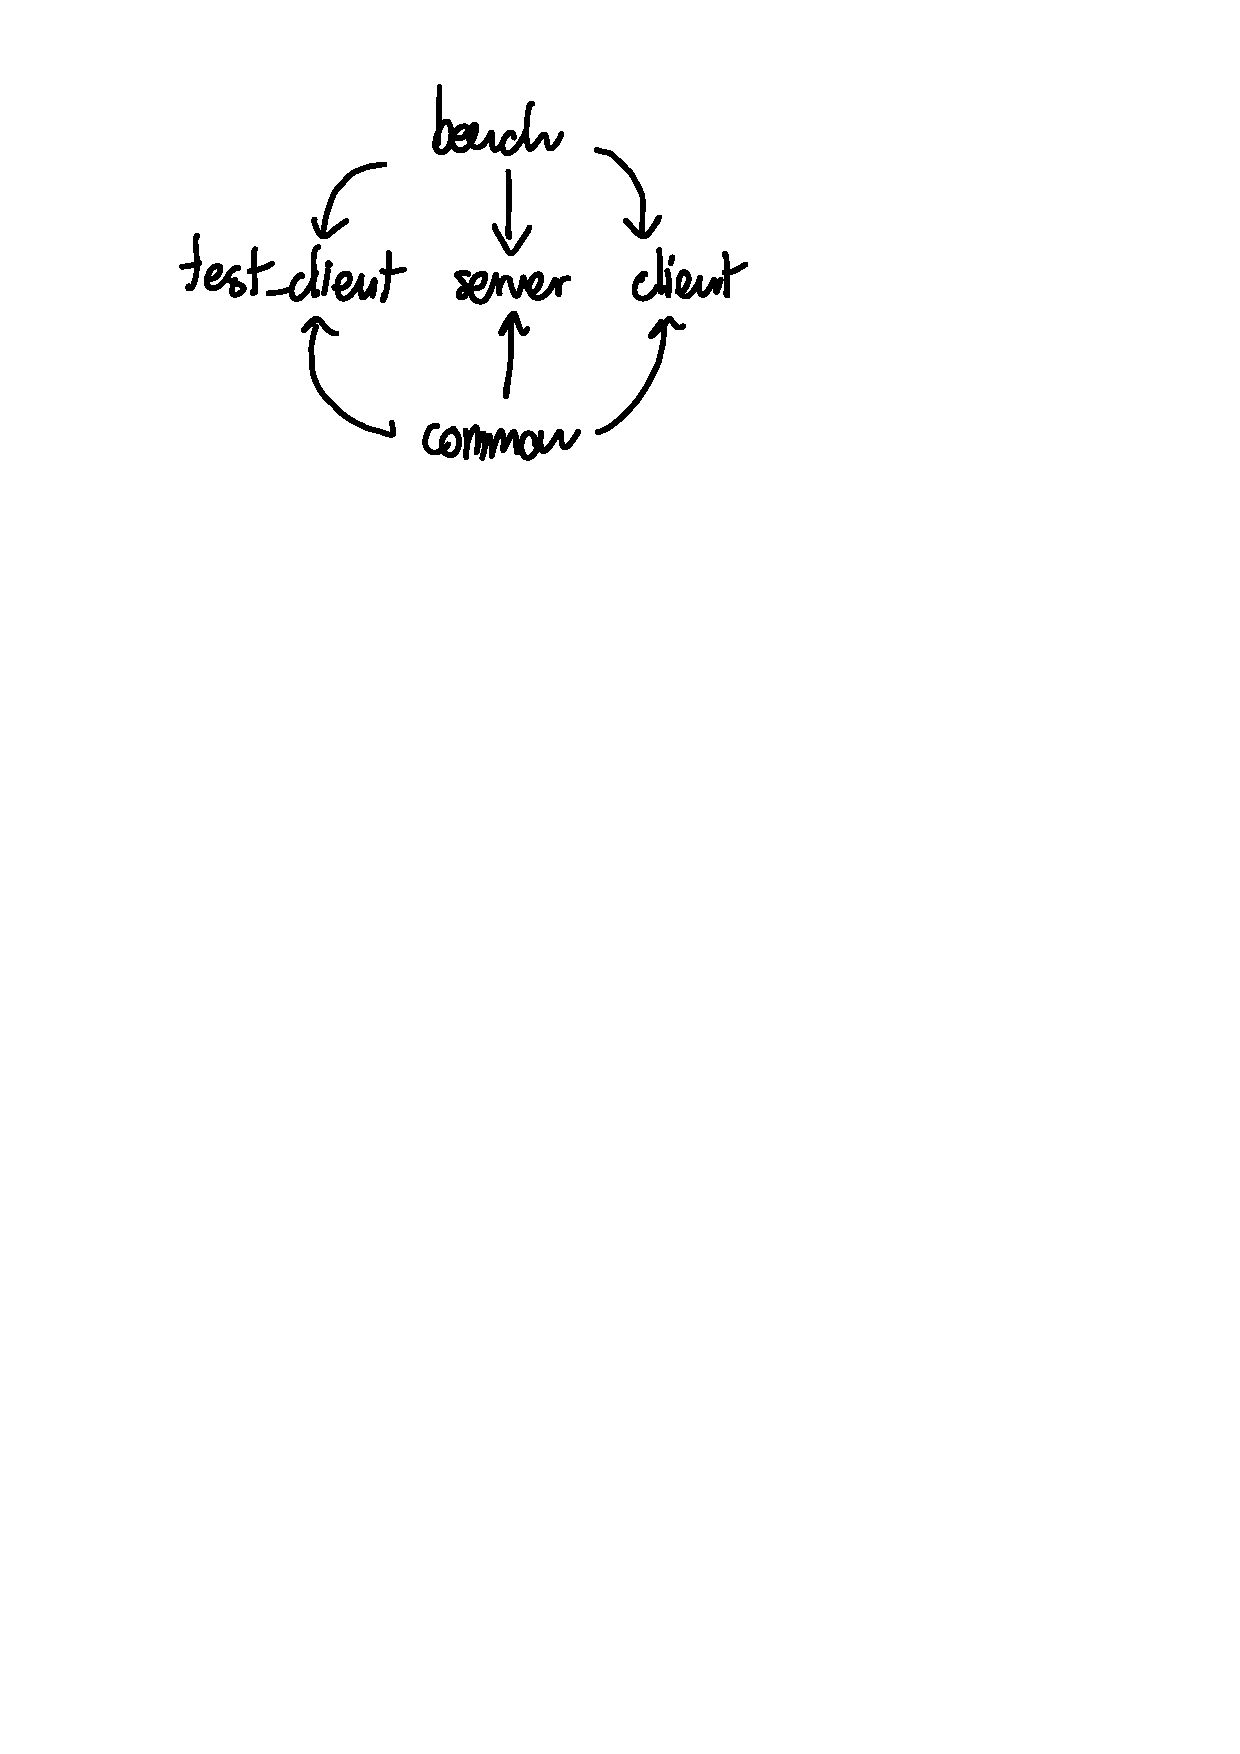
\includegraphics[width=\linewidth]{structure.pdf}
\end{mdframed}
\caption{\texttt{test\_client}, \texttt{server} and
\texttt{client} use the headers in \texttt{common} and
\texttt{bench}.}
\label{fig:folderdeps}
\end{figure}

Now \texttt{test\_client}, \texttt{server} and \texttt{client}
all contain source code which builds into their respective
binaries, those being the test client, the server and the client
respectively.

The \texttt{bench} folder contains all the necessary code to
facilitate benchmarking throughout the project. Of course,
benchmarking helps ensure adequate performance. More on this
later.

And finally, the \texttt{common} folder contains a number of
header files. These header files contain code which was either
immediately realised to be common (to all the three binaries) or
it was duplicated and then later refactored into
\texttt{common}.

\subsection{Scripts}

Throughout development a number of build configurations were
setup. As such scripts were written for using such
configurations. Additionally, some more complicated scripts were
also written.

In particular four different build scripts where created:

\begin{itemize}
    \item \texttt{build-json.sh},
    \item \texttt{build-rel.sh},
    \item \texttt{build-tsan.sh}, and
    \item \texttt{build.sh}.
\end{itemize}

\texttt{build.sh} and \texttt{build-rel.sh} are default builds,
but the first does not optimise (and includes debug information)
whilst the other optimises (and includes debug information). Of
course, in the event of an actual deployment
\texttt{build-rel.sh} should be used and stripping debug
information out should be considered.

\texttt{build-json.sh} is a debug build which enables the server
and any test client to dump there final draw vector as a JSON
file before exiting. This is of course useful to ensure that
proper synchronisation is indeed taking place among the clients
and the servers.

Finally, \texttt{build-tsan.sh} is again a debug build which
incorporates a thread sanitizer into our program. This can be
used to ensure that basic multithreading mistakes are avoided.

The next set of scripts is the following:

\begin{itemize}
    \item \texttt{client.sh},
    \item \texttt{client-debug.sh},
    \item \texttt{server.sh}, and
    \item \texttt{server-debug.sh}.
\end{itemize}

The above are all convenience scripts, they allow running the
binaries in \texttt{build/} directly from the project root.
Additionally, those which have the \texttt{-debug} suffix run
the binary inside \texttt{gdb} to allow for debugging.

The more interesting scripts are \texttt{stress-server.sh},
\texttt{stress-server-other-actions.sh} and
\texttt{collect-data.sh}. They facilitate stress testing the
server and collecting data about how the server performed. For
more information see Section \ref{sec:stresstesting}.

\section{Benchmarking}

A basic mechanism for benchmarking was developed. It is a single
header and single source file component and it manages a single
thread and a queue.

\begin{noteline}
    The benchmarking facility is only enabled by default for
    debug builds.
\end{noteline}

\begin{figure}[H]
\centering
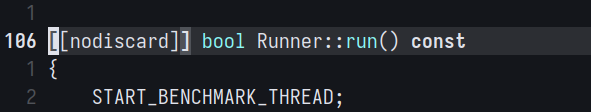
\includegraphics[width=\linewidth]{startingbenchmarkthread}
\caption{Starting the benchmark thread in
\texttt{src/server/runner.cpp} at line 108.}
\label{fig:startingbenchmarkthread}
\end{figure}

During initialisation the benchmarking thread can be started
using the \texttt{START\_BENCHMARK\_THREAD} macro (see Figure
\ref{fig:startingbenchmarkthread}). Then in the different areas
of the code which need to be tested, the macro
\texttt{BENCH("benchmark name")} can be used. The scope of the
benchmark is defined by RAII. \texttt{BENCH} keeps track of the
time at construction, and at destruction it calculates a time
delta.

\begin{attrib}
    The usage of RAII for the creation of scoped timers was
    heavily inspired by Yan Chernikov's guide to simple
    benchmarking, titled:
    \href{https://www.youtube.com/watch?v=YG4jexlSAjc}{BENCHMARKING
    in C++ (how to measure performance)} on YouTube.
\end{attrib}

\begin{figure}[H]
\centering
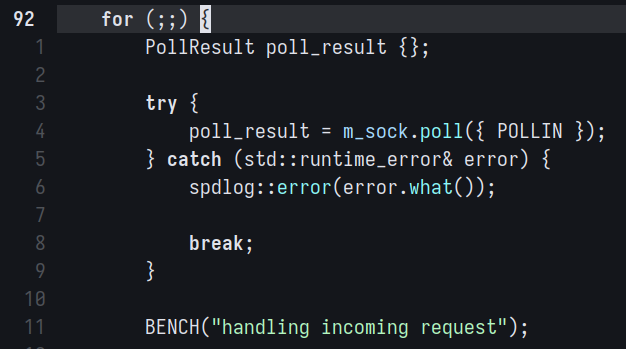
\includegraphics[width=\linewidth]{example-benchmark}
\caption{Example usage of the \texttt{BENCH} macro in the file
\texttt{src/server/server.cpp} at line 103.}
\label{fig:examplebenchmark}
\end{figure}

Now calling \texttt{BENCH("benchmark name")} by default will log
the result of the benchmark to the console. Additionally, it
will also enqueue the result as a pair \texttt{<"benchmark
name", \{Time Taken\}>} on the benchmark message queue. After
which, it notifies the benchmark thread.

\begin{note}
    The string used as a parameter to the \texttt{BENCH} macro
    uniquely identifies a specific benchmark. Additionally,
    calling \texttt{BENCH} multiple times with the same name
    will result in a moving average of the multiple readings
    (see Figure \ref{fig:serversidebenching}).
\end{note}

\begin{figure}[H]
\centering
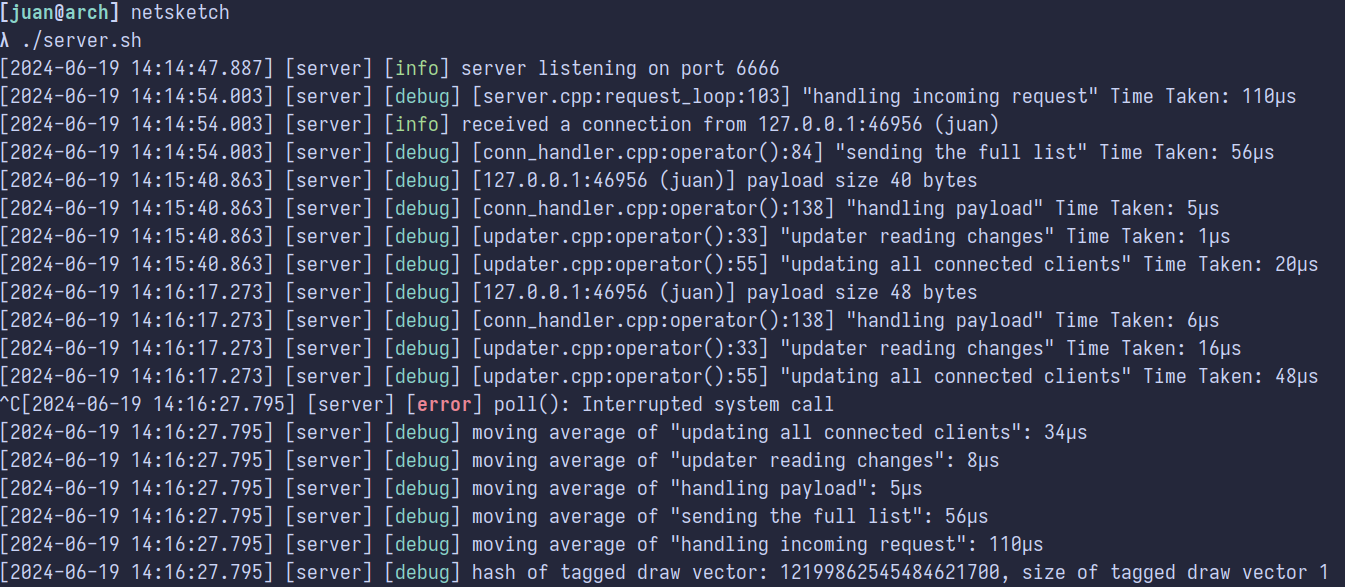
\includegraphics[width=\linewidth]{moving-average-example}
\caption{Example of server-side benchmarking (with logging).}
\label{fig:serversidebenching}
\end{figure}

Of course at the end of the program's life-time the benchmark
thread should be stopped with the macro
\texttt{END\_BENCHMARK\_THREAD}.

This part of the project is the backbone which facilitates the
work done in Section \ref{sec:stresstesting}.

\section{Common Headers}

\begin{figure}[H]
\centering
\begin{mdframed}[backgroundcolor=OffWhite]
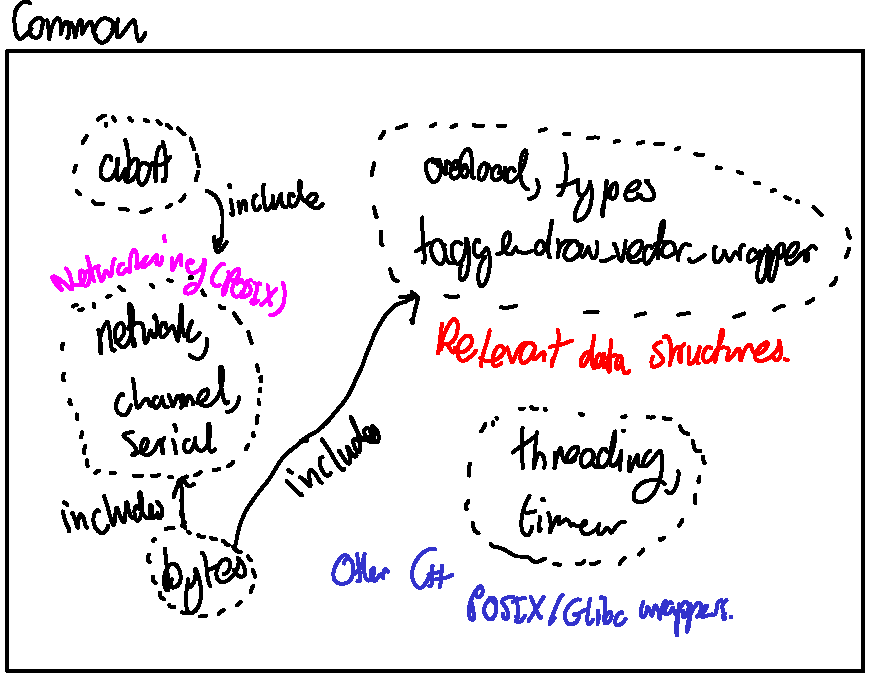
\includegraphics[width=\linewidth]{common-groupings}
\end{mdframed}
\caption{Logical groupings of the files in the common folder.}
\label{fig:commongroups}
\end{figure}

There are a number of logical groupings in in the common folder
(see Figure \ref{fig:commongroups}). The smallest of which are
\texttt{abort.hpp} and \texttt{bytes.hpp}. \texttt{bytes.hpp}
only contains an alias to \texttt{std::string} called
\texttt{ByteString}.

\begin{figure}[H]
\centering
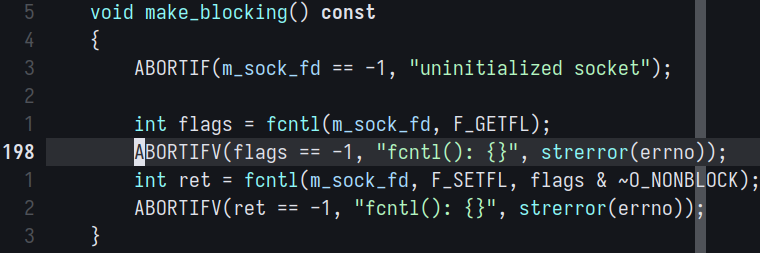
\includegraphics[width=\linewidth]{abort-usage}
\caption{Usage of the \texttt{ABORTIF} and \texttt{ABORTIFV}
(variadic variant) macros in \texttt{src/common/network.hpp} at line
195.}
\label{fig:abortusage}
\end{figure}

\subsection{Abort}

\texttt{abort.hpp} provides some crucial functionality. In
particular, it provides mechanisms for abruptly terminating the
program. This is useful because there are states that the
program should never reach. It should not even be allowed to be
in an error state. If such states are indeed reached the program
should abort (see Figure \ref{fig:abortusage}).

\subsection{Relevant Data Structures (Types)}

\begin{figure}[H]
\centering
\begin{mdframed}[backgroundcolor=OffWhite]
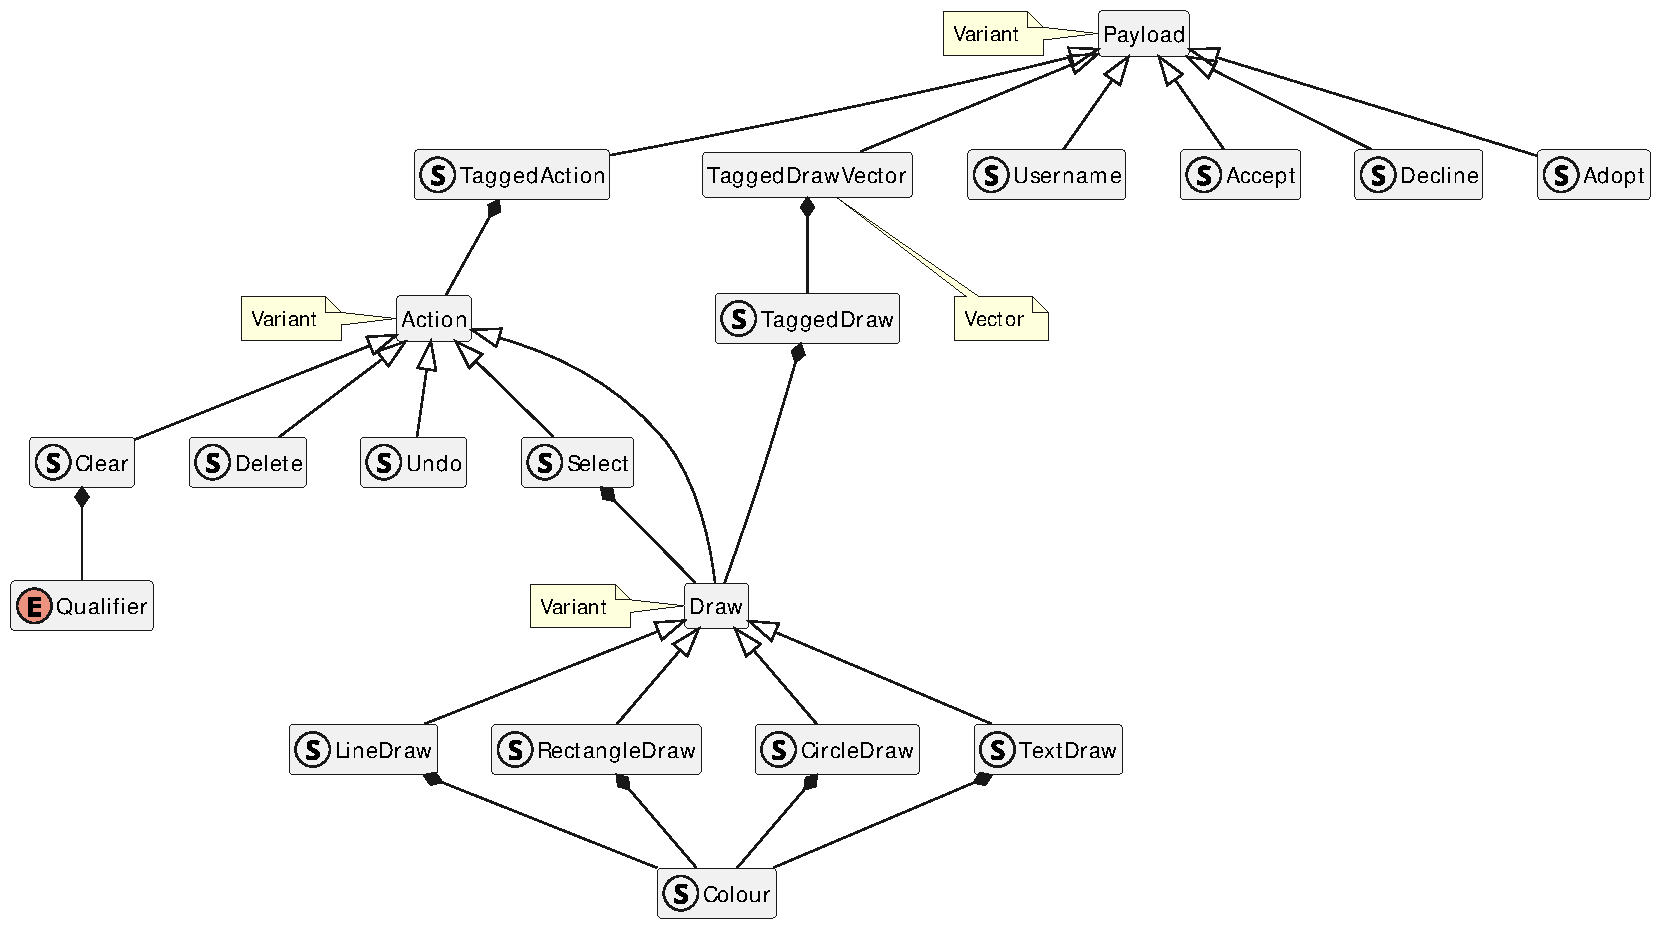
\includegraphics[width=\linewidth]{types.pdf}
\end{mdframed}
\caption{A hierarchy of all the types relevant to the
functionality of the whiteboard (in the
\texttt{src/common/types.hpp} file).}
\label{fig:typetree}
\end{figure}

The \texttt{types.hpp} file contains all the relevant data types
which the server, test client and client use (see Figure
\ref{fig:typetree}). The \texttt{overload.hpp} file contains
some helpers which facilitate more concise and functional syntax
for dealing with \texttt{std::variant} types (for an example see
\texttt{src/client/gui.cpp}, line 93).

\begin{note}
    A \texttt{Payload} can be a \texttt{TaggedAction}. This
    allows the system to send over deltas or partials instead of
    sending the full modified state every time the server
    receives an updated.
\end{note}

The \texttt{tagged\_draw\_vector\_wrapper.hpp} contains a class
which wraps a tagged draw vector, essentially augmenting the
tagged draw vector with the manipulations (e.g. deleting a
specific draw command) required by the project specification.

\subsection{Networking (POSIX)}

The \texttt{serial.hpp} file contains easier interfaces for
serialising and de-serialising than those provided by cereal.

The \texttt{network.hpp} file contains abstractions around C's
POSIX networking primitives. The abstractions allow for safer
code by taking advantage of RAII. In particular, the most
important part of the file is the \texttt{IPv4Socket} class. It
creates a significantly easier interface for interacting with
sockets.

Additionally, the comment above the \texttt{IPv4SocketRef} class
is important because it validates the need for such a shell
class. In summary, it allows sockets to be copied and moved with
being destroyed due to RAII.

The \texttt{channel.hpp} file contains the main Channel class.
The class wraps around an socket reference and it allows for a
simpler approach to over-the-network communication.

\begin{figure}[H]
\centering
\begin{bytefield}[bitwidth=1.5em,bitheight=2.6em]{10}
\bitheader{0-9} \\
\bitbox{2}{\scriptsize\texttt{0x2003}} & \bitbox{8}{Payload Size (Bytes)}
\end{bytefield}
\caption{A diagram of the structure of a NetSketch header.}
\label{fig:netsketch-header}
\end{figure}

This is because the class automatically wraps any binary string
into a packet which is comprised of a header and a payload. The
header contains a few two initial bytes which identify the
packet as a NetSketch packet and then it contains an 8-byte
integer, which indicates how many more bytes should be read.

\begin{marker}
    The size field is critical for receiving the full message.
    This is because, the socket interface requires that the
    number of bytes to be read is provided. This means that the
    number of bytes a receiver needs to read has to be either
    fixed or an initial segment of a known fixed size is sent
    which contains the size of the actual message.
\end{marker}

Additionally, the methods within the Channel class always return
a \texttt{ChannelErrorCode} as part of there return type. This
forces the users of channels to properly handle errors and do so
in a neater way instead of using \texttt{errno} (and everything
related to it directly).

\subsection{Other \CC{} POSIX/\texttt{glibc}
Wrappers}\label{sec:posixwrappers}

The \texttt{threading.hpp} file is a large collection of \CC{}
wrappers around the threading primitives provided by POSIX. The
reason for this is detailed in the beginning of the file.
However, the key take away is that the STL does not provide
first class support for all the features provided by the POSIX
standard. In particular, the most important feature is
cancelability (the ability to direct the kernel to stop a
thread). Although \texttt{std::thread} does use the underlying
primitive of its platform abusing this fact and mixing POSIX
threads and STL threads seems inapt. Hence, an effort was made
to copy the parts of the STL necessary for work, whilst at the
same time ensuring 100\% compatibility with POSIX.

\begin{figure}[H]
\centering
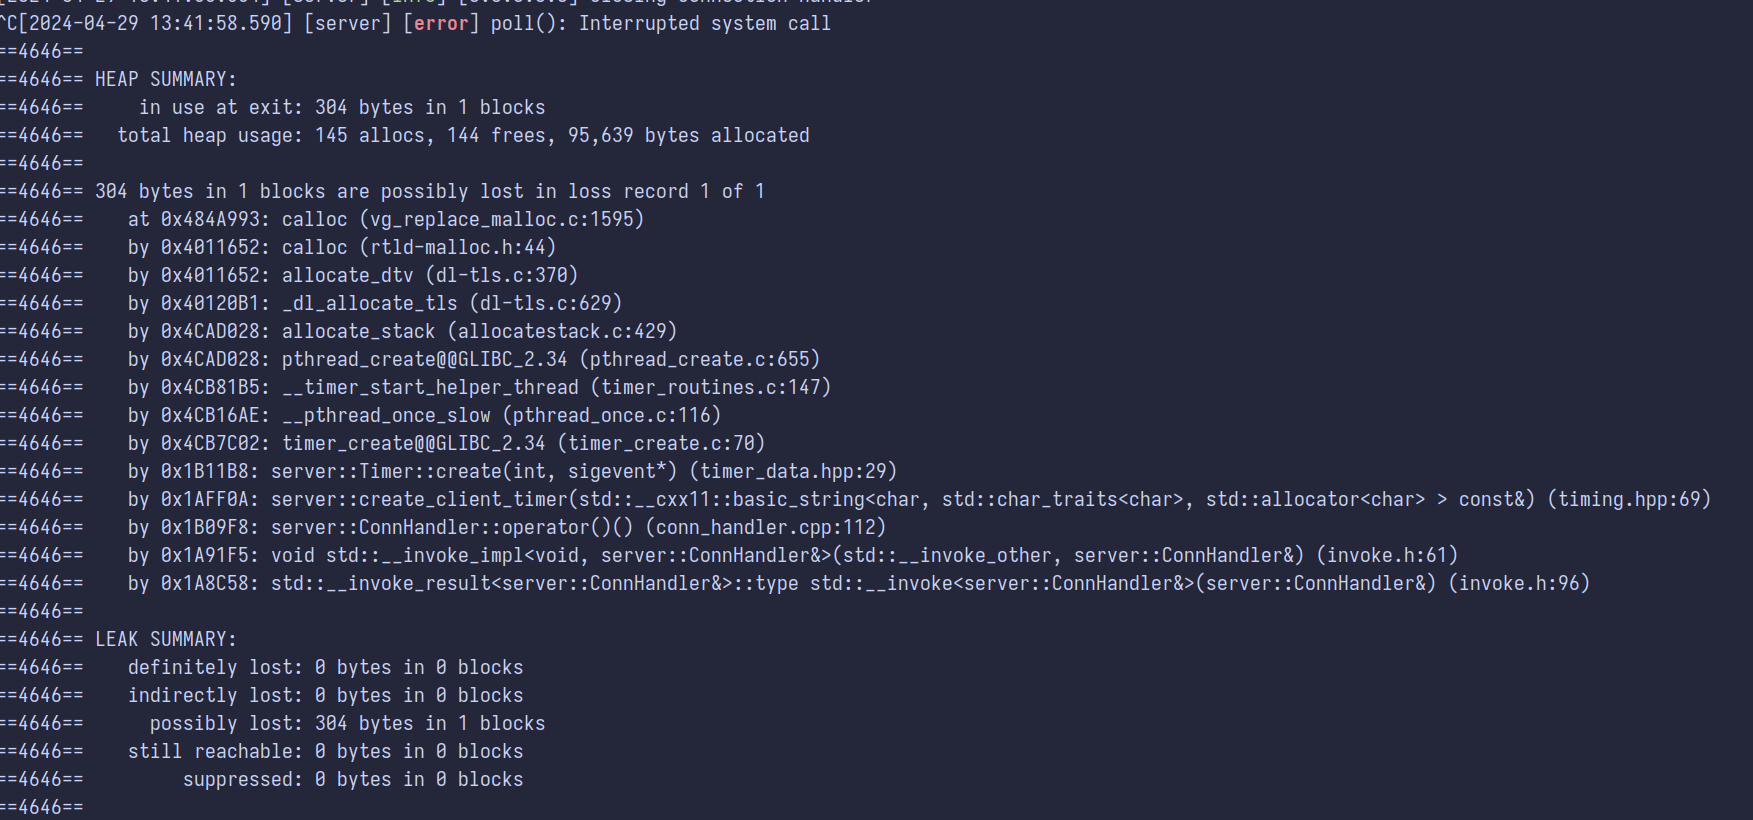
\includegraphics[width=\linewidth]{timer-leak}
\caption{Running \texttt{valgrind} on the server binary to test
for memory leaks.}
\label{fig:timerleak}
\end{figure}

Finally, the \texttt{timer.hpp} file similarly wraps around the
timer mechanisms provided by \texttt{glibc} providing a \CC{}
interface which makes use of RAII.

\begin{note}
    \texttt{glibc} timers are being used instead of a custom
    solution to reduce code complexity and reduce the need for
    managing additional threads (which are used as timers).
    Instead \texttt{glibc} manages these automatically. However,
    the only downside to this approach is the fact
    \texttt{glibc} always leaks a single allocation (see Figure
    \ref{fig:timerleak}).
\end{note}

\section{The Client}

\begin{note}
    \raggedright
    A demonstration of the client can be seen in the video
    presentation hosted here:
    \url{https://drive.google.com/file/d/1VMXR4Z0s5iDvXcroMTLn6ddb5enplOTF/view?usp=drive_link}.
\end{note}

\subsection{Shared State}

The approach used for cross-thread communication was shared
state. To achieve this a \texttt{share.hpp} file was used to
contain all the variables which needed to exist outside and
hence between threads.

This most includes the majority of used synchronisation
primitives such as mutexes, condition variables and read-write
locks. Additionally, it contains any threads handles, queues and
vectors which need to be global or are used for communication
between one thread and another.

\subsection{Client Thread Structure}

\begin{figure}[H]
\centering
\begin{mdframed}[backgroundcolor=OffWhite]
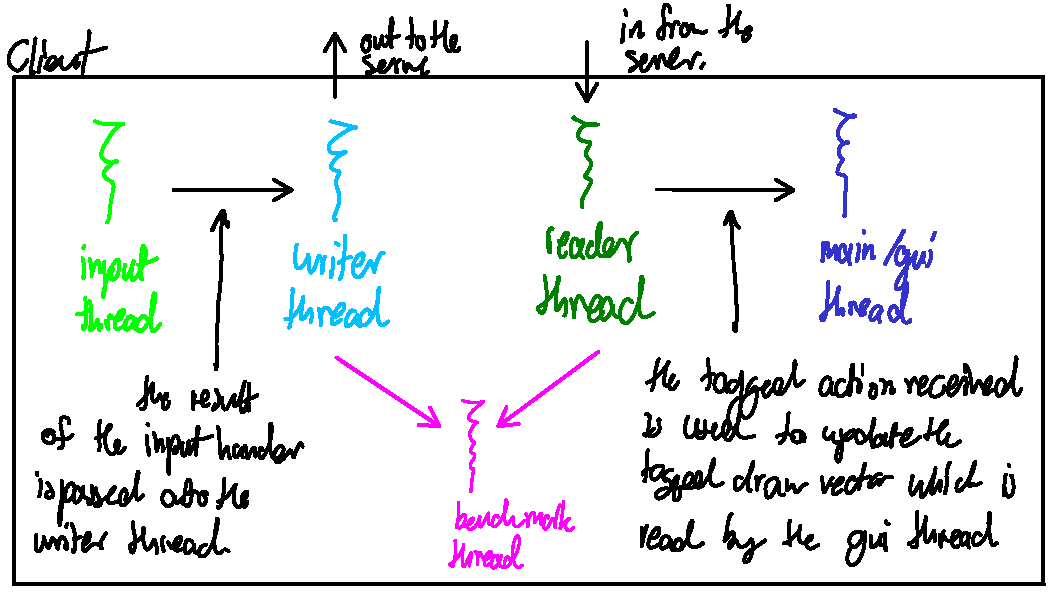
\includegraphics[width=\linewidth]{client-thread-structure}
\end{mdframed}
\caption{A drawing of the threads and their interactions in the
client binary.}
\label{fig:clientthreads}
\end{figure}

The above Figure \ref{fig:clientthreads}, gives an adequate
depiction of the thread interaction in the client. Expanding a
bit, the input thread, generally interacts with the writer
thread using the writer queue and, its associated mutex and
condition variables (see \texttt{src/client/share.hpp} lines
23-25).

The Reader-GUI communication is the more complicated of the two.
This is because the camera of the GUI can be managed
independently from the client's command line interface. This
imposes the following restriction: \emph{the GUI should allow
for a smooth user experience even if a whiteboard update is
incoming}.

This means that the canvas or GUI should never freeze up during
an update.

\begin{figure}[H]
\centering
\begin{mdframed}[backgroundcolor=OffWhite]
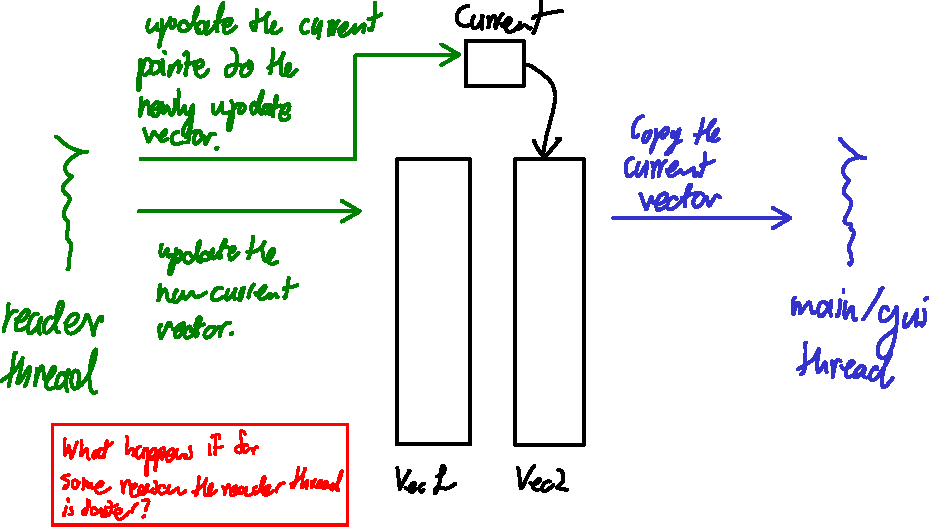
\includegraphics[width=\linewidth]{reader-gui-comms}
\end{mdframed}
\caption{A drawing of the initial double-buffering technique
employed to ensure responsiveness.}
\label{fig:readerguicomms}
\end{figure}

The main approach for tackling this problem is to use a
technique knowing as double buffering. This is most commonly
used in graphics related scenarios. A simple implementation
should have two vectors which are always in parity but are
maintained independently. Whilst a pointer called `current' is
used to indicate which of the vectors the GUI thread should read
from.

At any point in time the reader thread can update the unused
vector. Then after finishing the `current' pointer is updated by
the reader and the other vector is also updated, at which point
the `current' pointer is swapped again.

However, this approach and specifically trying to avoid the use
of synchronisation primitives (as they are very expensive) led
to a race condition.

\subsection{Reader-GUI Race Condition (+ Solution)}

\begin{figure}[H]
\centering
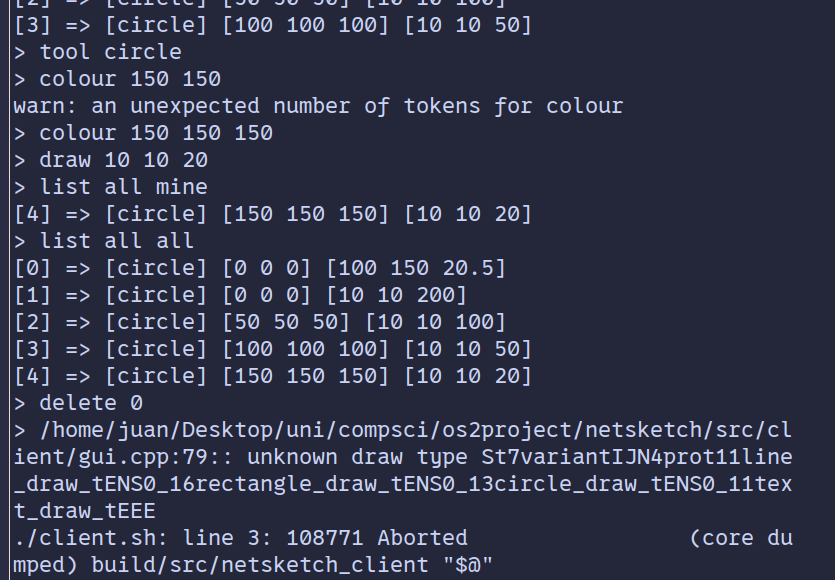
\includegraphics[width=\linewidth]{original-data-race}
\caption{An abnormal exit of the program caused by an unknown
type, later verified to be caused by a data race.}
\label{fig:originaldatarace}
\end{figure}

After some digging and research it was later verified to be an
issue caused by a data race as indicated by Figure
\ref{fig:readerguicomms}. In particular, it was happening
because the reader was sometimes faster than the GUI and whilst
the GUI was reading, the reader would update the underlying
structure. Because of this, the GUI would momentarily read
malformed data leading to an abnormal exit (as seen in Figure
\ref{fig:originaldatarace}).

Additionally, the issue was appearing irregularly since it is
not very common for the GUI thread to be slower than the reader
thread. However, to confirm the issue the GUI was artificially
slowed downed using a sleep. This confirmed the issue and that
it was caused due a timing issue between the reader and GUI
threads.

\begin{figure}[H]
\centering
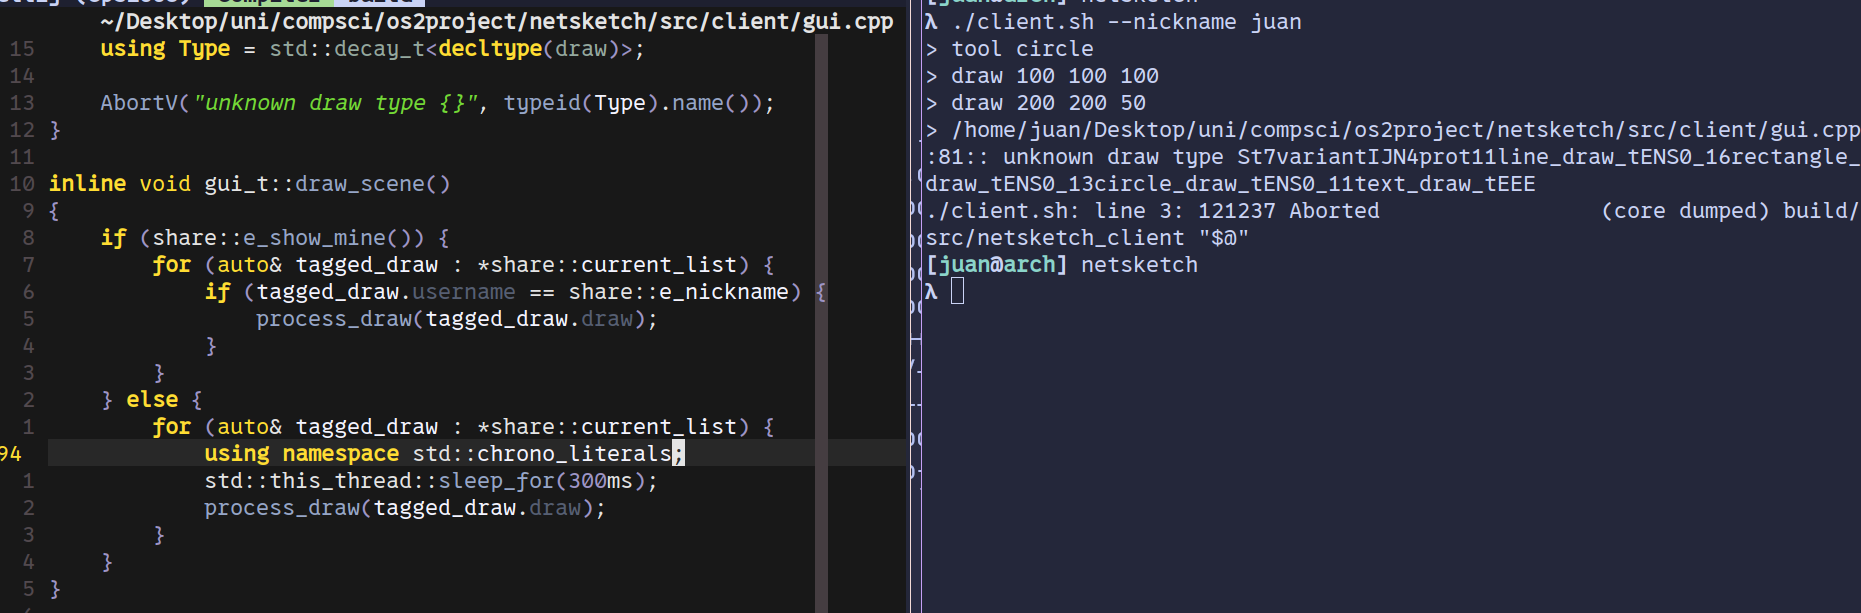
\includegraphics[width=\linewidth]{artificial-data-race}
\caption{Artificially inducing the data race exhibited in Figure
\ref{fig:originaldatarace} using a sleep function.}
\label{fig:artificialdatarace}
\end{figure}

After some research the following article was found:
\url{http://concurrencyfreaks.blogspot.com/2013/11/double-instance-locking.html}.
The author(s) claim that the technique is ``lock-free'' for
(in our case) the GUI thread, which is exactly what was needed to
still ensure responsiveness. Implementing there described
approach solved the issue.

\begin{marker}
    Performance before and after the change was not measured.
    This is because of a number of reasons. In particular, the
    infrastructure for benchmarking was not yet present in the
    project and correctness takes precedence over speed.
\end{marker}

\section{The Server}

\subsection{Shared State}

With regards to the sharing of state between threads a similar
approach to what was used within the client is also being used
within the server. The only difference is that within the server
there are more globally shared variables due to the server being
overall more complex (see \texttt{src/server/share.hpp}).

\subsection{Server Thread Structure}

\begin{figure}[H]
\centering
\begin{mdframed}[backgroundcolor=OffWhite]
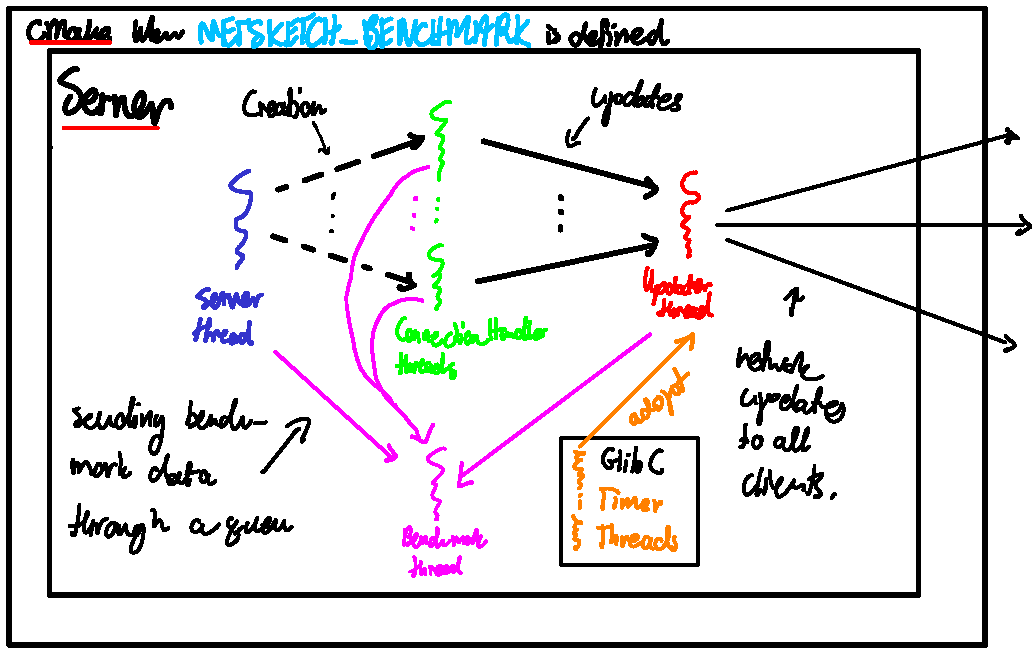
\includegraphics[width=\linewidth]{threadinteractions-server.pdf}
\end{mdframed}
\caption{A drawing of all the thread interactions in the
server.}
\label{fig:serverthreads}
\end{figure}

The threads present within the server are the server thread, the
updater, thread the connection handler threads and the timer
threads.

In particular, the server thread sets up the necessary
networking and handles new incoming connections. When a new
connection arrives a connection handler thread is created to
handle that specific user. Further communications from the
client are handled by its respective connection handler.

Each connection handler then interacts with the updater thread
which updates the local state of the server and sends the same
update to all the connected clients.

The timer threads are managed by \texttt{glibc} and there main
purpose is to give a disconnected user a time gap before his
draw commands are adopted by the server.

\subsection{Limitations of the Updater Model}\label{subsec:updatermodel}

The main problem with the current model is the fact the that the
updater thread is a bottleneck. If sufficiently many clients are
connected to the server, it will take the updater more time to
finish every next update cycle, since it has to send the update
to all the connected users in a for-loop.

However, solving this problem is not easy. Using a
Publisher-Subscriber model seems adequate however, it will still
have the same bottleneck as the current model if internally
somewhere a for-loop is notifying each thread.

To solve a problem like this a design which inverts the
responsibility of staying notified is required. However, this
also has its own drawbacks. Will the threads all continuously
poll to check if an update is present? Unfortunately, there does
not seem to be an elegant solution which maintains code
complexity to a minimum. Because of this fact the initial
solution was kept.

\subsection{Other Server Behaviours}

\subsubsection{Abrupt Server Termination}

\begin{figure}[H]
\centering
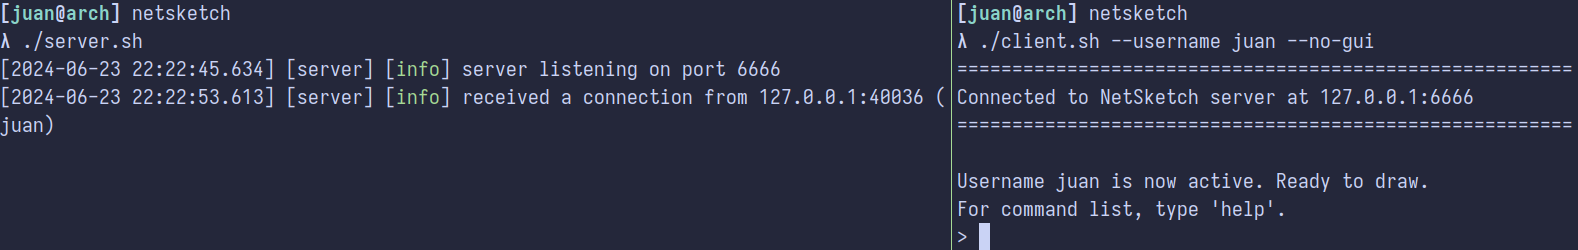
\includegraphics[width=\linewidth]{normal-setup}
\caption{A screenshot of a operational server and client.}
\label{fig:normalsetup}
\end{figure}

\begin{figure}[H]
\centering
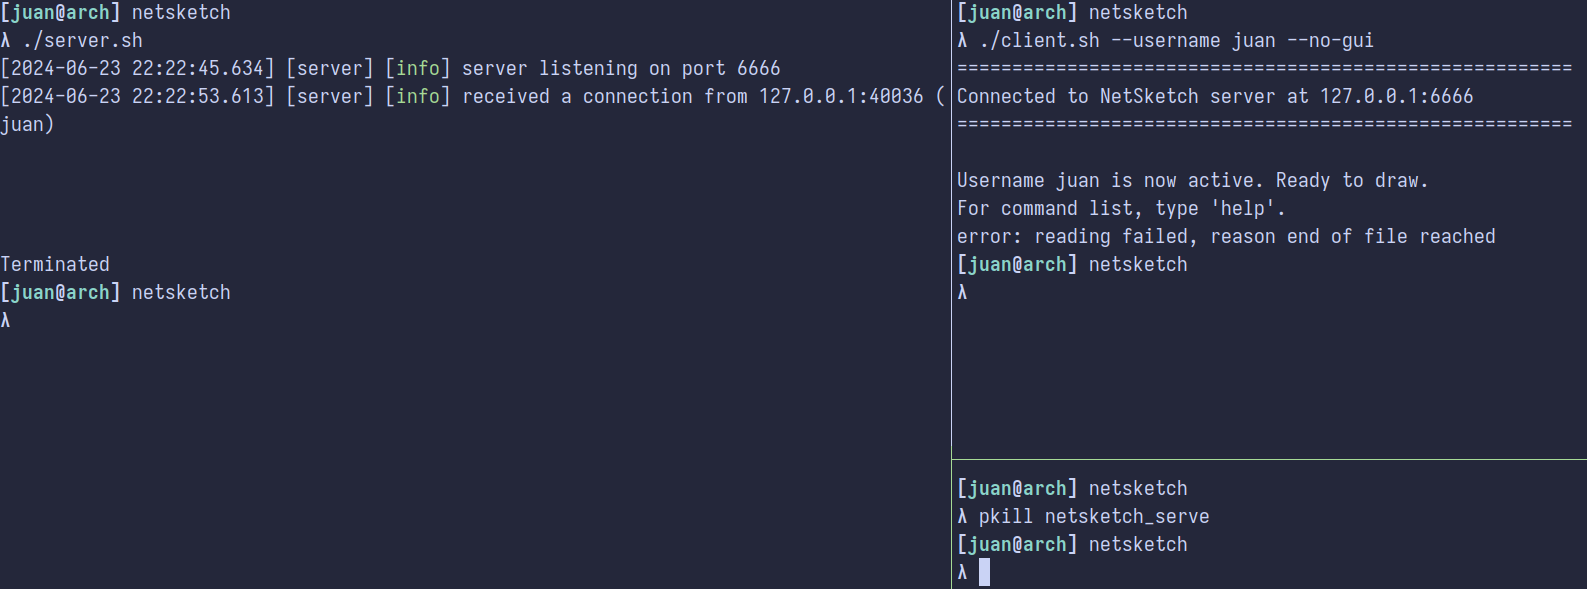
\includegraphics[width=\linewidth]{abrupt-termination-of-server}
\caption{A screenshot of a artificially induced termination
(using \texttt{pkill}).}
\label{fig:abrupttermination}
\end{figure}

In the event that the server abruptly terminates, all connected
clients also terminate (see Figure \ref{fig:abrupttermination}).

\subsubsection{Disconnecting Idle Users}

\begin{figure}[H]
\centering
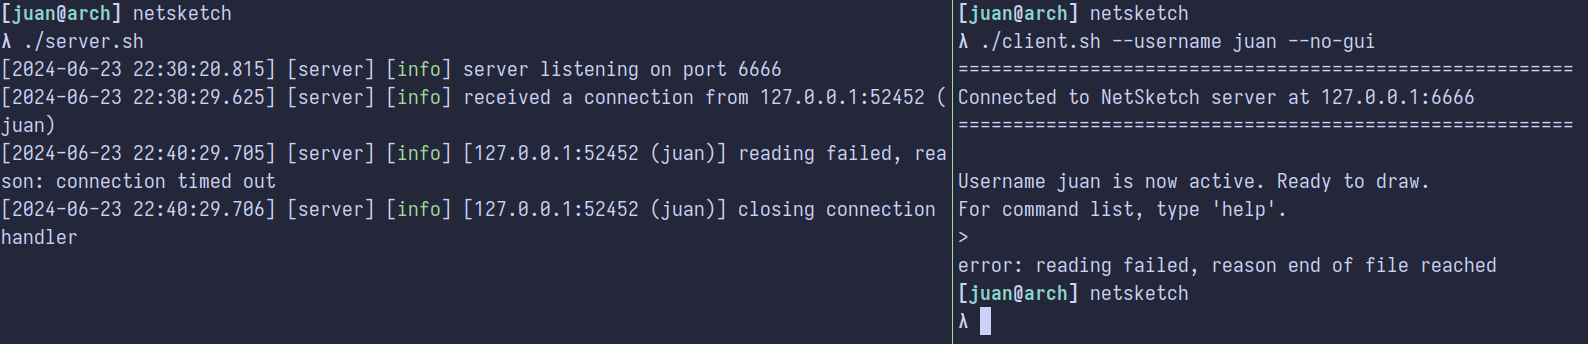
\includegraphics[width=\linewidth]{disconnected-user}
\caption{A screenshot of a server disconnecting a user that has
been idle for ten minutes.}
\label{fig:idleuser}
\end{figure}


\begin{figure}[H]
\centering
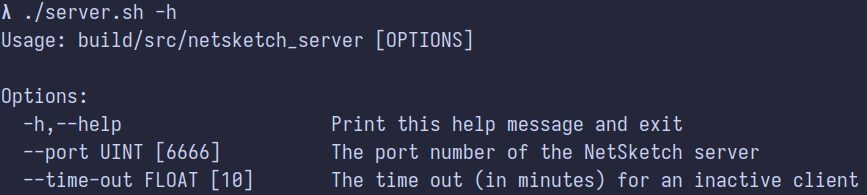
\includegraphics[width=\linewidth]{server-help}
\caption{A screenshot of the server's help menu.}
\label{fig:serverhelp}
\end{figure}

The server can disconnect idle clients. The default timeout is
set to ten minutes. However, this can be changed to any number
of minutes (see Figure \ref{fig:serverhelp}).

\subsubsection{Draw Call Adoption}

\begin{figure}[H]
\centering
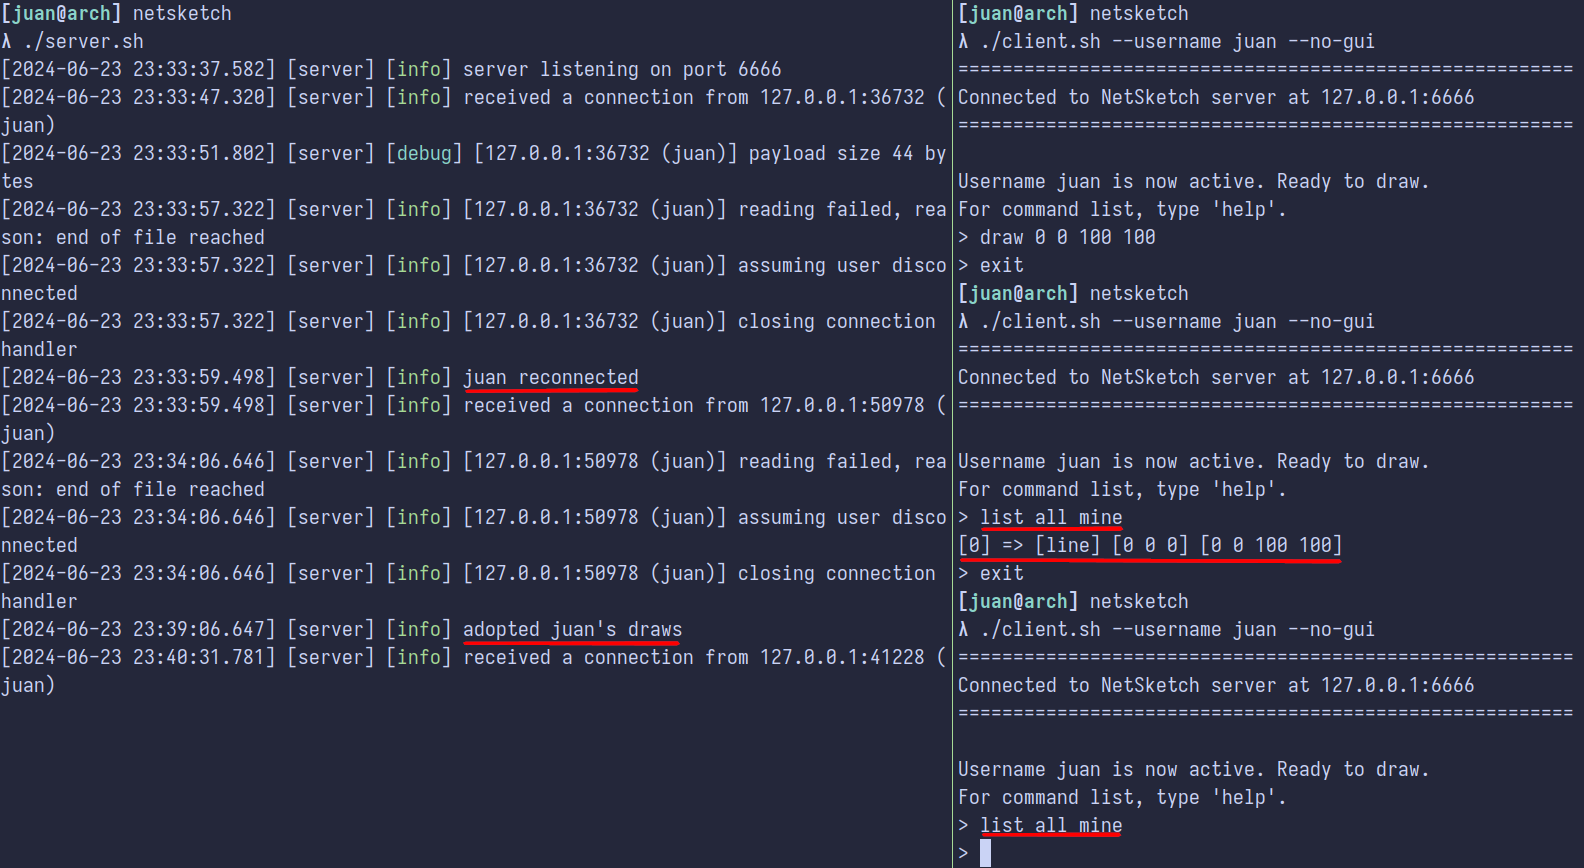
\includegraphics[width=\linewidth]{adoption-example}
\caption{A screenshot demonstrating draw command adoption by the
server (the relevant server logs and client info if
highlighted).}
\label{fig:useradoption}
\end{figure}

When a client disconnects the server preserves the user's
ownership of his/her draw commands for five minutes. After
that the server adopts the commands and if a user connects
they'll no longer have ownership of those draw commands.

In the event that a client unexpectedly disconnects, this
approach gives the client a buffer to reconnect without losing
their progress and hence continue where they left off.

\subsubsection{Clashing Usernames}

\begin{figure}[H]
\centering
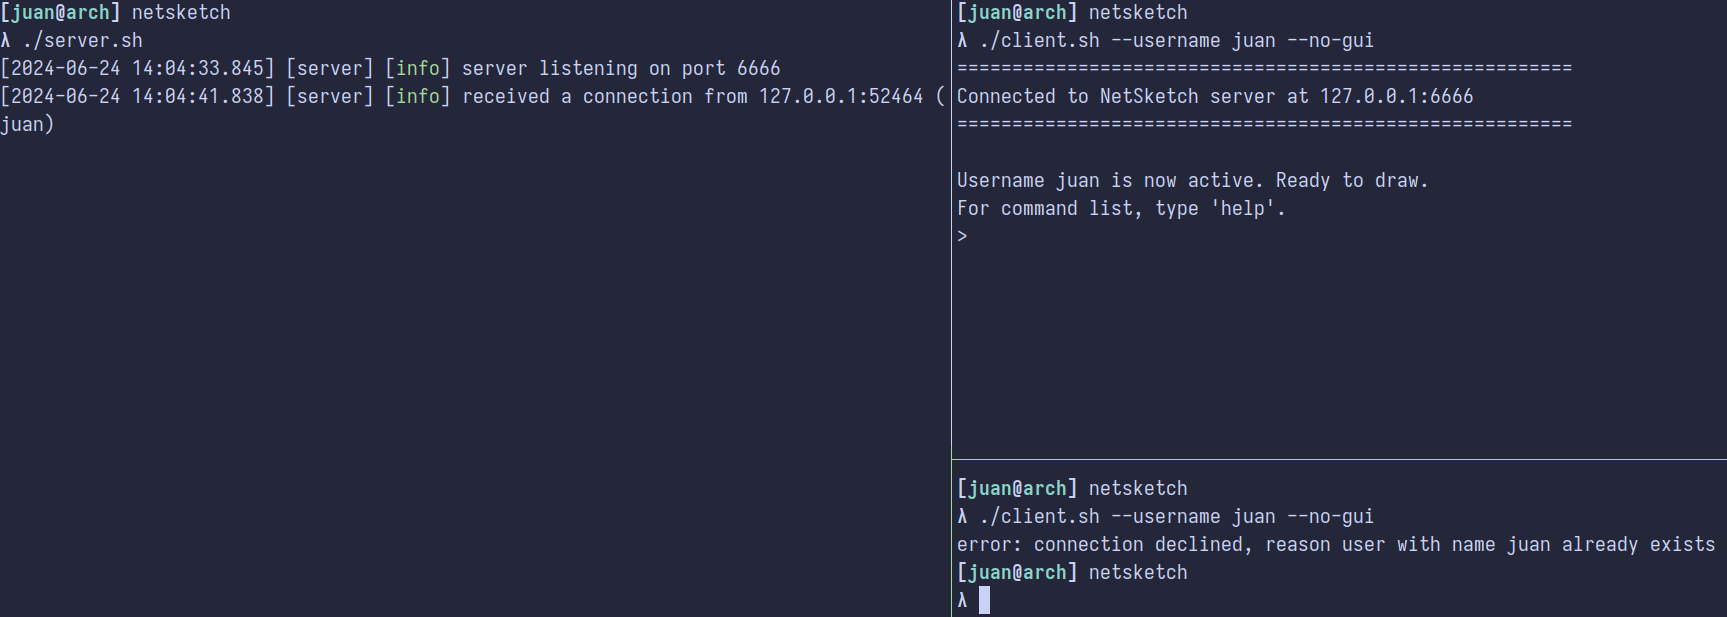
\includegraphics[width=\linewidth]{username-clash}
\caption{A screenshot two clients requesting the same name. One
of the clients is refused by the server.}
\label{fig:useradoption}
\end{figure}

For every possible username the server only supports a single
connection.

\section{The Test Client}

The test client is a variation of the actual client. It
takes in as input the following extra command line arguments:

\begin{itemize}
    \item \texttt{--iterations} which is the number of requests
        the test client will send to the server,
    \item \texttt{--interval} which is the interval in between
        each request in seconds,
    \item \texttt{--expected\_responses} which is
        \textbf{suppose} to be the total number of responses the
        test client will receive (however it refers to the total
        number of expected draw commands), and
    \item \texttt{--other\_actions} which indicates whether
        generating undo, select and clear should be allowed or
        not.
\end{itemize}

\begin{marker}
    The \texttt{--expected\_responses} flag's behaviour is
    prefixed by a `\textbf{suppose}'. This is because it was
    realised that calculating the number of expected responses
    especially, if multiple test clients are present is
    extremely difficult. This is the case because if multiple
    tests clients are present some will actually connect to the
    server later than others. This means that they will receive
    all the changes events up to that point as one whole tagged
    draw vector i.e. one response. Hence, calculating the number
    of expected responses is impossible. Instead the number of
    expected responses actually refers to the number of draw
    calls or the final expected size of the tagged draw vector.
    Additionally, note that if the other actions were also
    enabled it would also make the calculation impossible.
\end{marker}

The \texttt{--expected\_responses} flag is important because it
tells the test client when to stop and terminate. In the event
that the quota set by the \texttt{--expected\_responses} flag is
never met, the test client will wait until the server
automatically, disconnects the client due to inactivity (circa
ten minutes).

The most critical behaviour of a test client is its generation
of random actions which is contained in the file
\texttt{src/test\_client/simulate\_user.cpp}. It is a simple
for-loop which uniformly generates all the available drawing
commands (if the \texttt{--other\_actions} flag is set it will
generate all actions uniformly).

\subsubsection{Thread Structure}

The thread structure of the test client is similar to the normal
client except it does not have a dedicated input thread and the
GUI/main is used for running the above mentioned random
action/draw generator.

\section{Stress/Performance Testing}\label{sec:stresstesting}

\subsection{Testing the Server}

Now having established a test client, the scripts
\texttt{stress-server.sh} and
\texttt{stress-server-other-actions.sh} can be used to , of
course, stress the server and test for correctness.

Additionally, the \texttt{collect-data.sh} script can be used to
gather information about the server, in particular, its
performance under heavy load.

\subsubsection{Testing Correctness}

\begin{figure}[H]
\centering
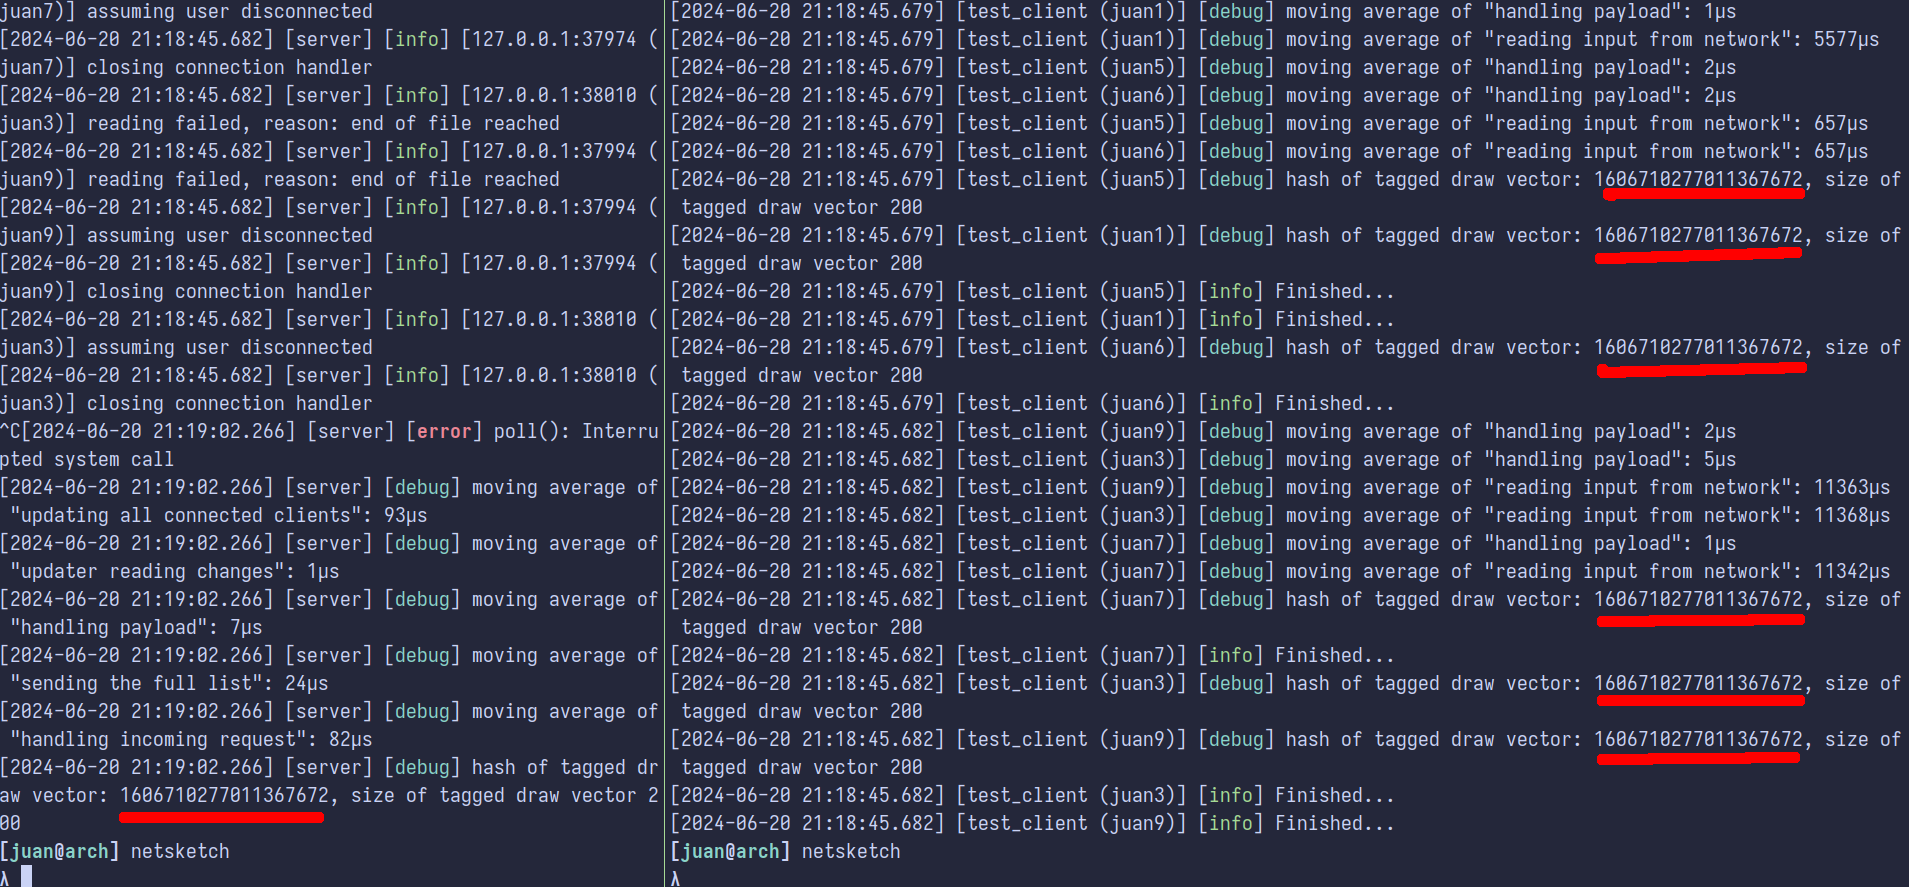
\includegraphics[width=\linewidth]{stress-server-10-20-0.5}
\caption{Stressing the server with ten test clients and twenty
draw commands at an interval of 0.5 seconds (with the tagged
draw vector hashes highlighted).}
\label{fig:stresstest1}
\end{figure}

\begin{note}
    Under debug builds the tagged draw vector can be hashed.
    This allows us to compare the hashes generated by the
    different test clients and the server.
\end{note}

When testing for correctness an initial stress test using the
debug build is performed. This stress tests yields the hashes of
the tagged draw vectors held by each test client and the server
(see Figure \ref{fig:stresstest1}).

These hashes can then be compared. Any discrepancies are
indicative of issues with correctness, specifically
synchronisation.

\begin{figure}[H]
\centering
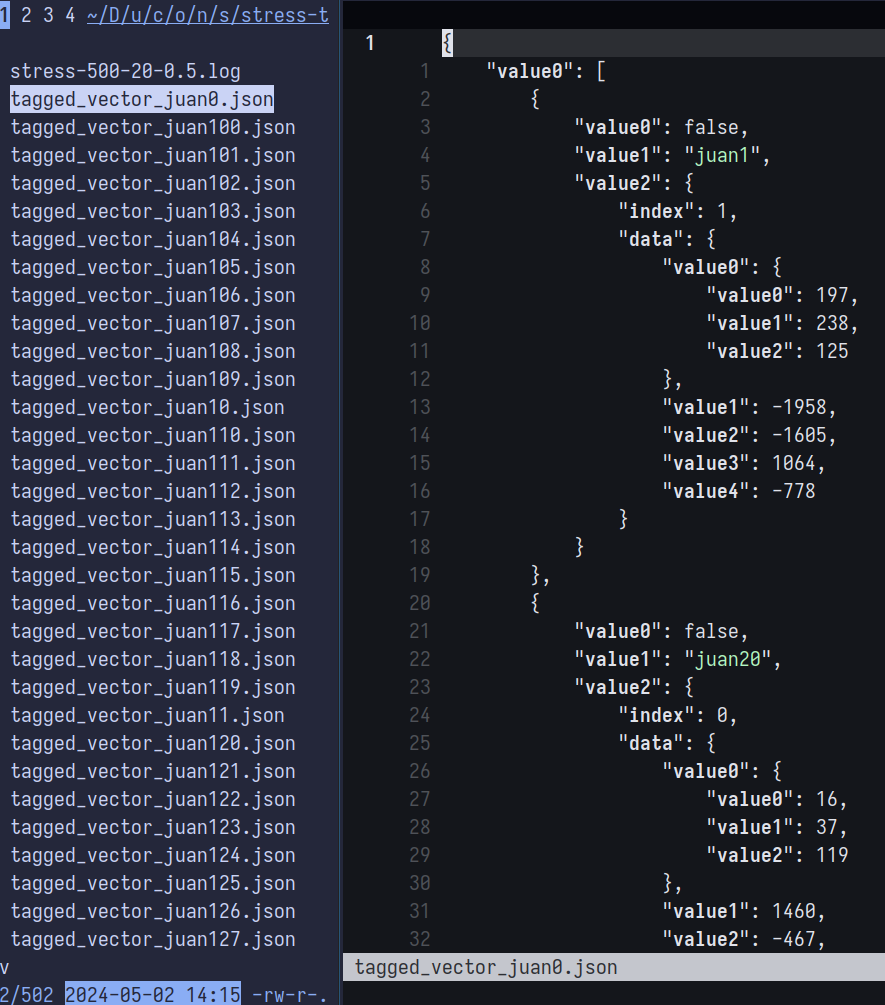
\includegraphics[width=\linewidth]{tagged-vector-json-dumps-2}
\caption{A collection of JSON dumps along with an open JSON file.}
\label{fig:jsondump}
\end{figure}

In the event that two or more of these hashes are different, the
binaries can be recompiled with \texttt{build-json.sh}. This
allows each of the test clients and the server to dump their
local tagged draw vector as a JSON file. These files can then be
manually inspected.

Of course, this does not guarantee an easier time debugging
however, it can provide insight as to why the observed behaviour
is being recorded.

\begin{figure}[H]
\centering
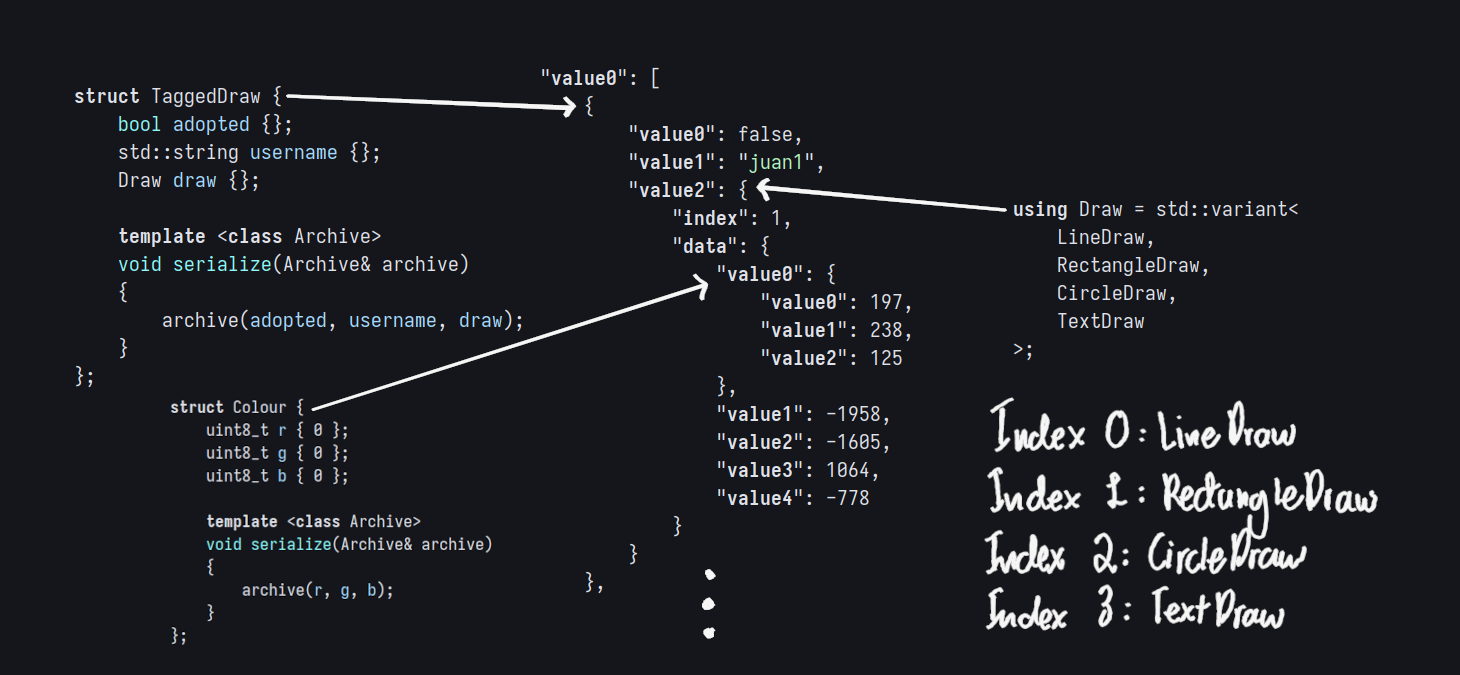
\includegraphics[width=\linewidth]{json-guide}
\caption{A graphical guide to understanding a dumped JSON file.}
\label{fig:jsondumpguide}
\end{figure}

\begin{note}
    The dumped JSON files (see Figure \ref{fig:jsondump}) lack
    proper names for the fields. This is because the cereal
    serialisation library only supports the addition of such
    names when serialising into XML or JSON. However, the
    program is also serialising into portable binary making it a
    bit more difficult to annotate fields with names.  Please
    see Figure \ref{fig:jsondumpguide} for a guide on reading
    the JSON files.
\end{note}

\begin{figure}[H]
\centering
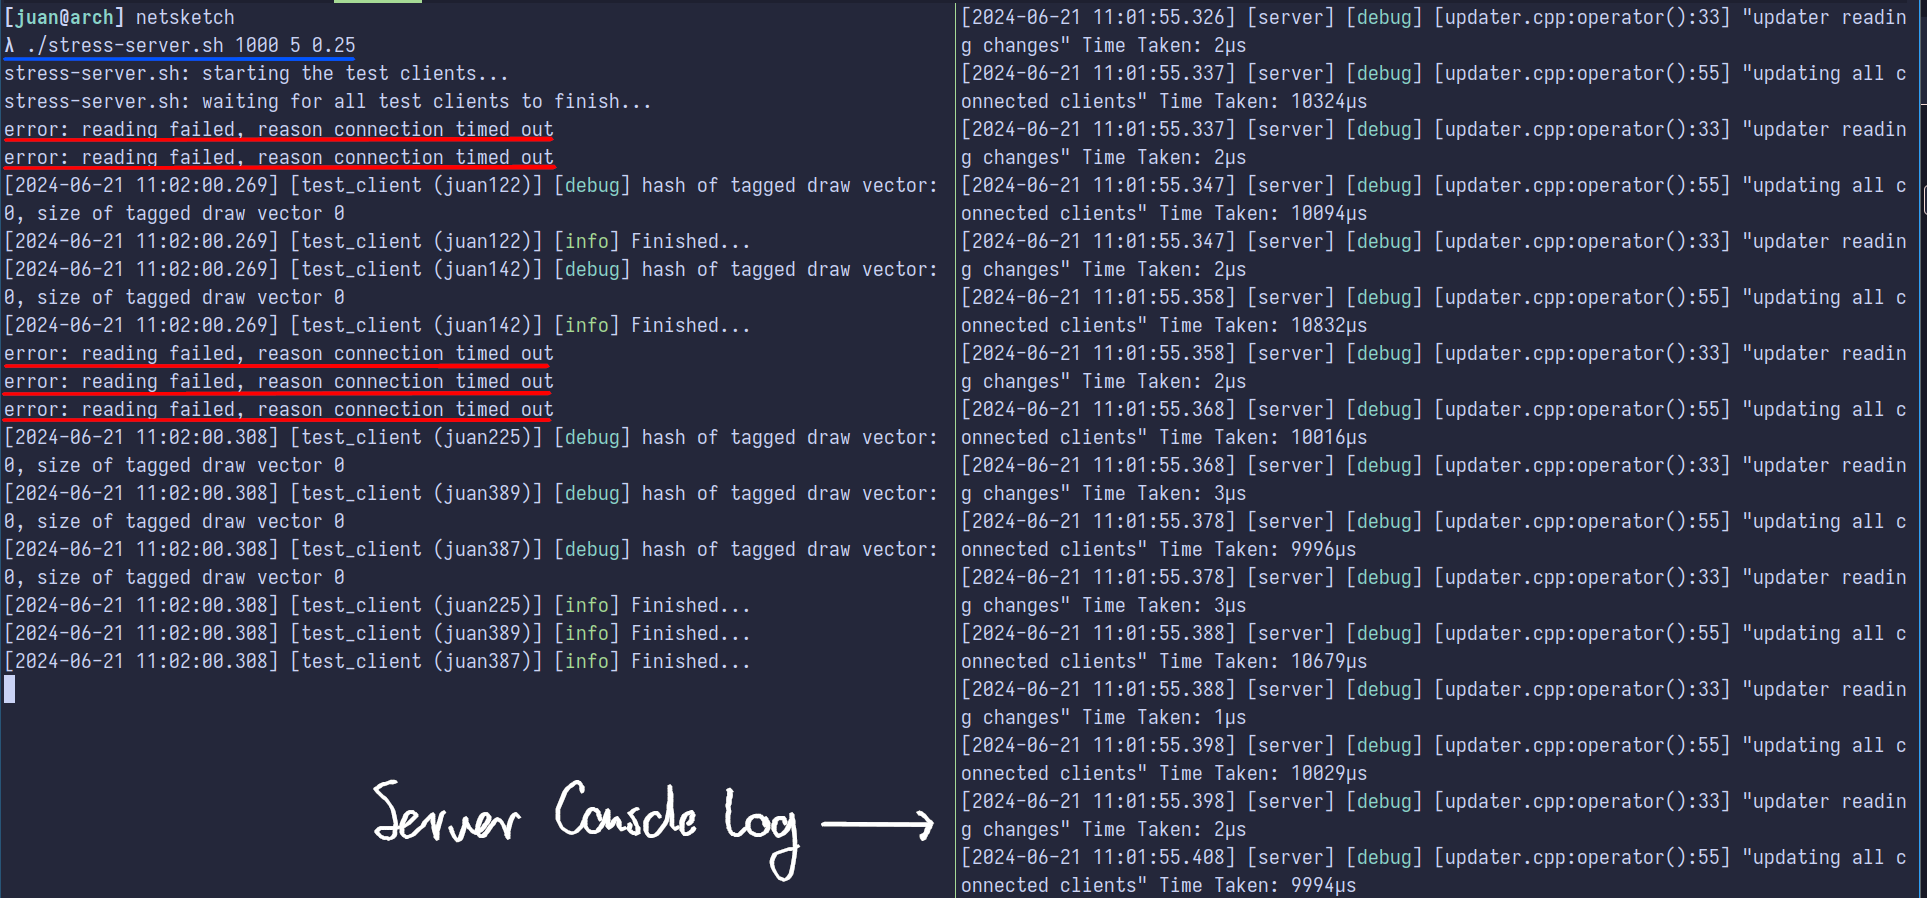
\includegraphics[width=\linewidth]{difficult-stress-initial.png}
\caption{Initial phase of a stress test with 1000 test clients
(the command and timeout errors are highlighted).}
\label{fig:initial1000stress}
\end{figure}

\begin{figure}[H]
\centering
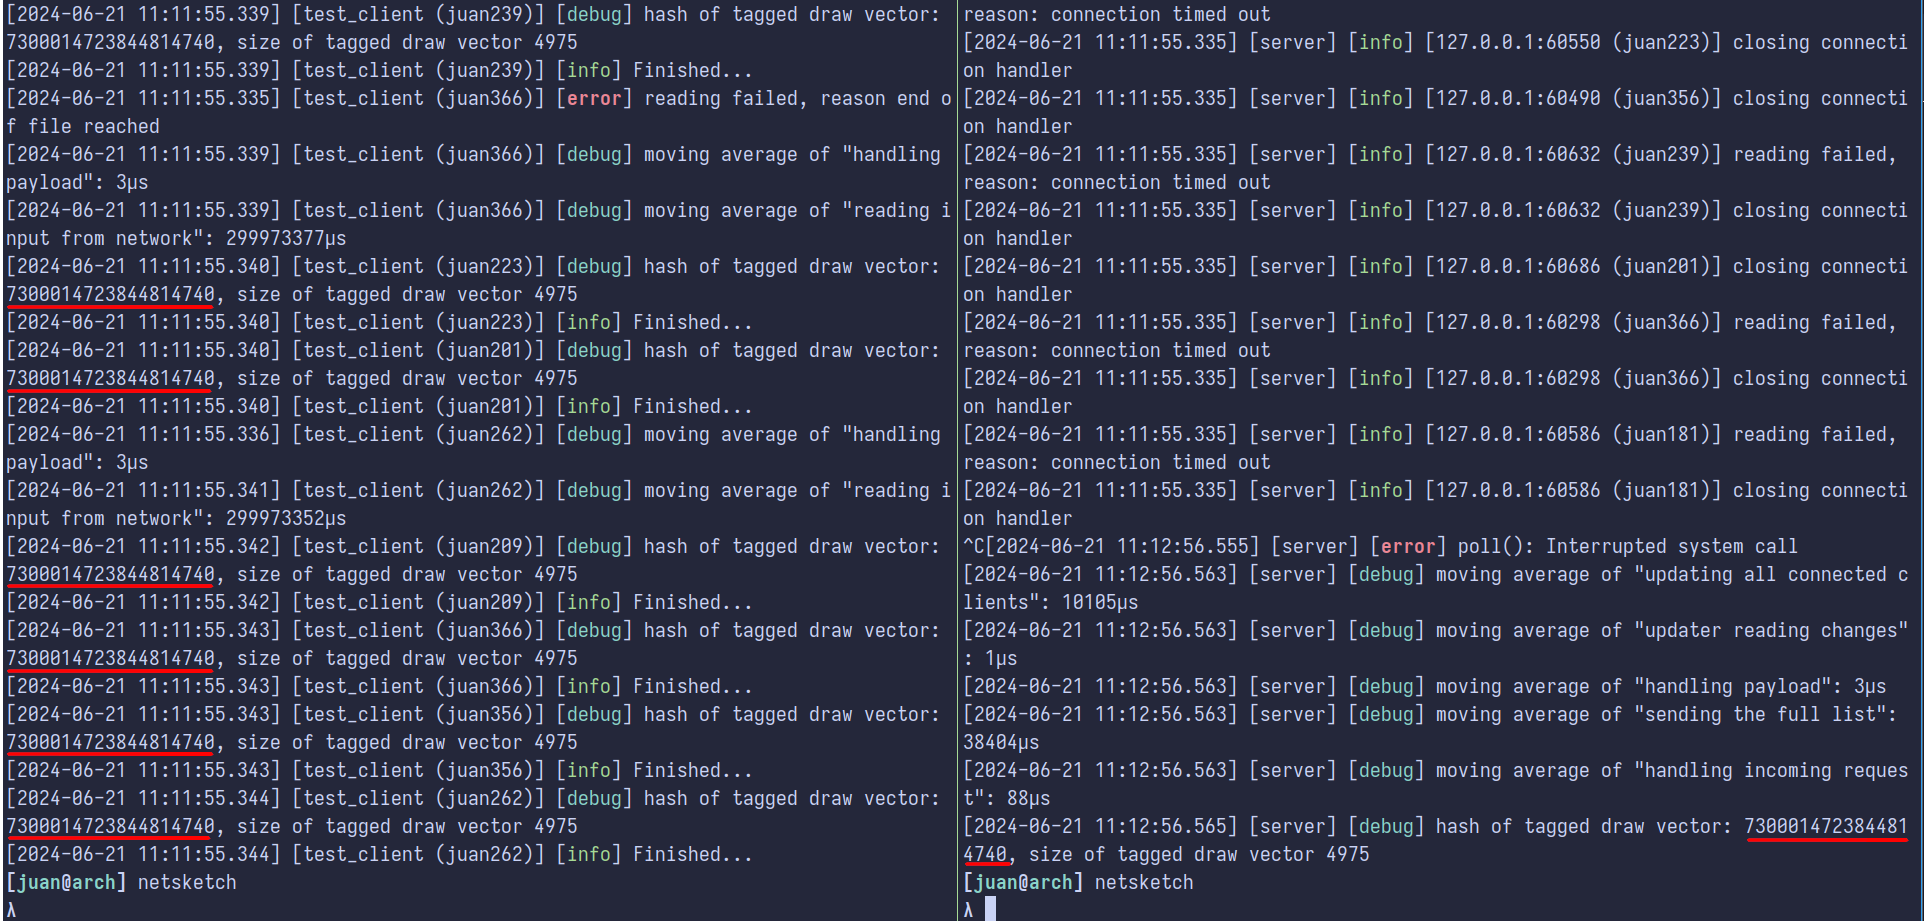
\includegraphics[width=\linewidth]{difficult-stress-end.png}
\caption{End phase of a stress test with 1000 test clients (the
tagged draw vector hashes are highlighted).}
\label{fig:end1000stress}
\end{figure}

Currently, the project only starts to exhibit issues with
correctness when 1000 simultaneous test clients try to connect
to the server. However, this only seems to be a networking
limitation, since some of the connections (see Figure
\ref{fig:initial1000stress}) are dropped. Because of this the
test clients do not automatically terminate, since they do not
reach their expected draw count. However, after ten minutes of
idling the server automatically, disconnects the clients.

At the end (see Figure \ref{fig:end1000stress}) it still seems
that overall the server's mechanisms for synchronisation are
robust. This is because the hashes produced from the tagged draw
vectors still seem to be equal to one another.

\begin{figure}[H]
\centering
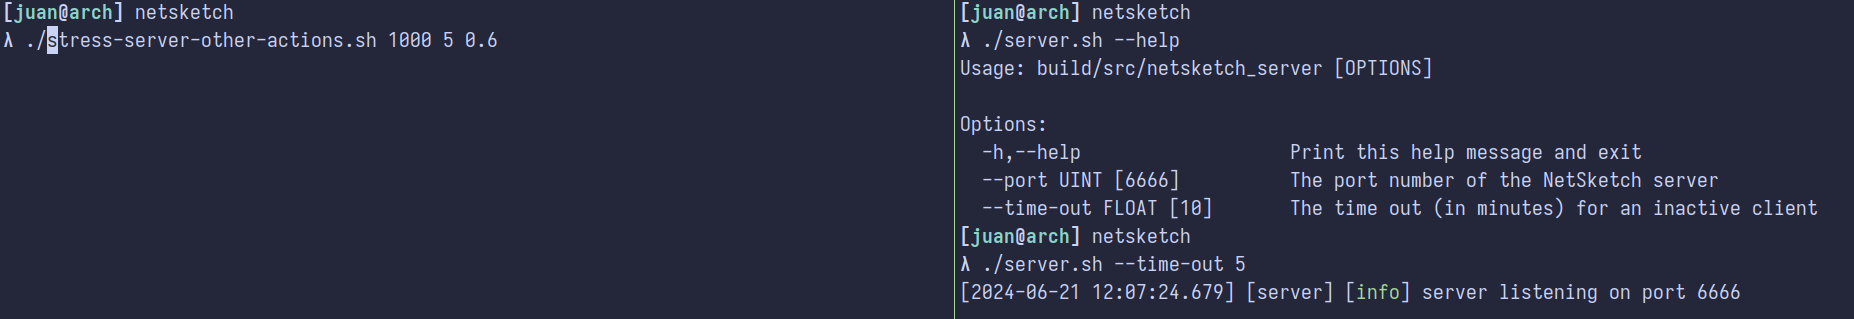
\includegraphics[width=\linewidth]{difficult-stress-other-start.png}
\caption{Start of a stress test with 1000 test clients (with
other actions enabled and the tagged vector hashes
highlighted).}
\label{fig:start1000stressother}
\end{figure}

\begin{figure}[H]
\centering
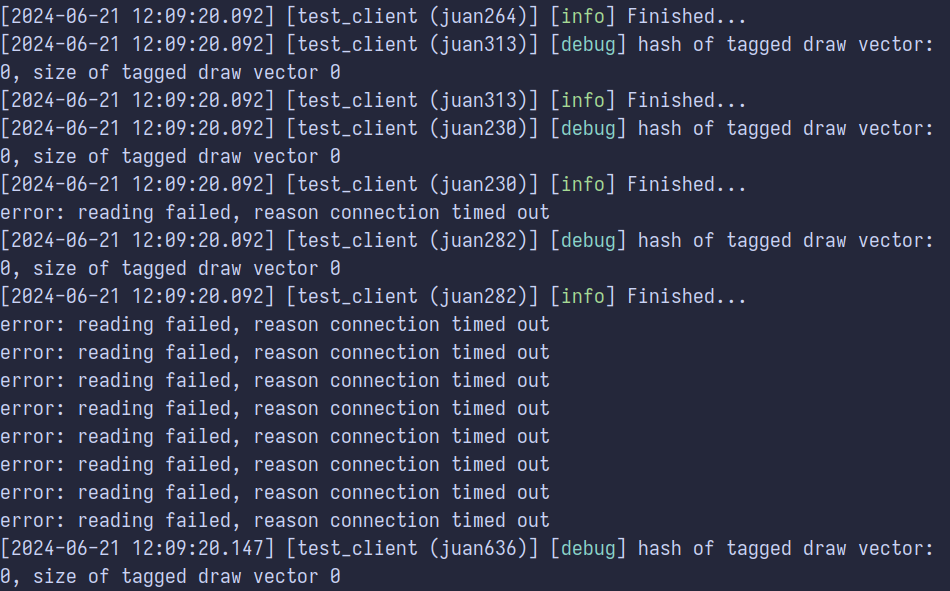
\includegraphics[width=\linewidth]{difficult-stress-other-timeout.png}
\caption{Some test clients again experience timeout errors.}
\label{fig:timeout1000stressother}
\end{figure}

\begin{figure}[H]
\centering
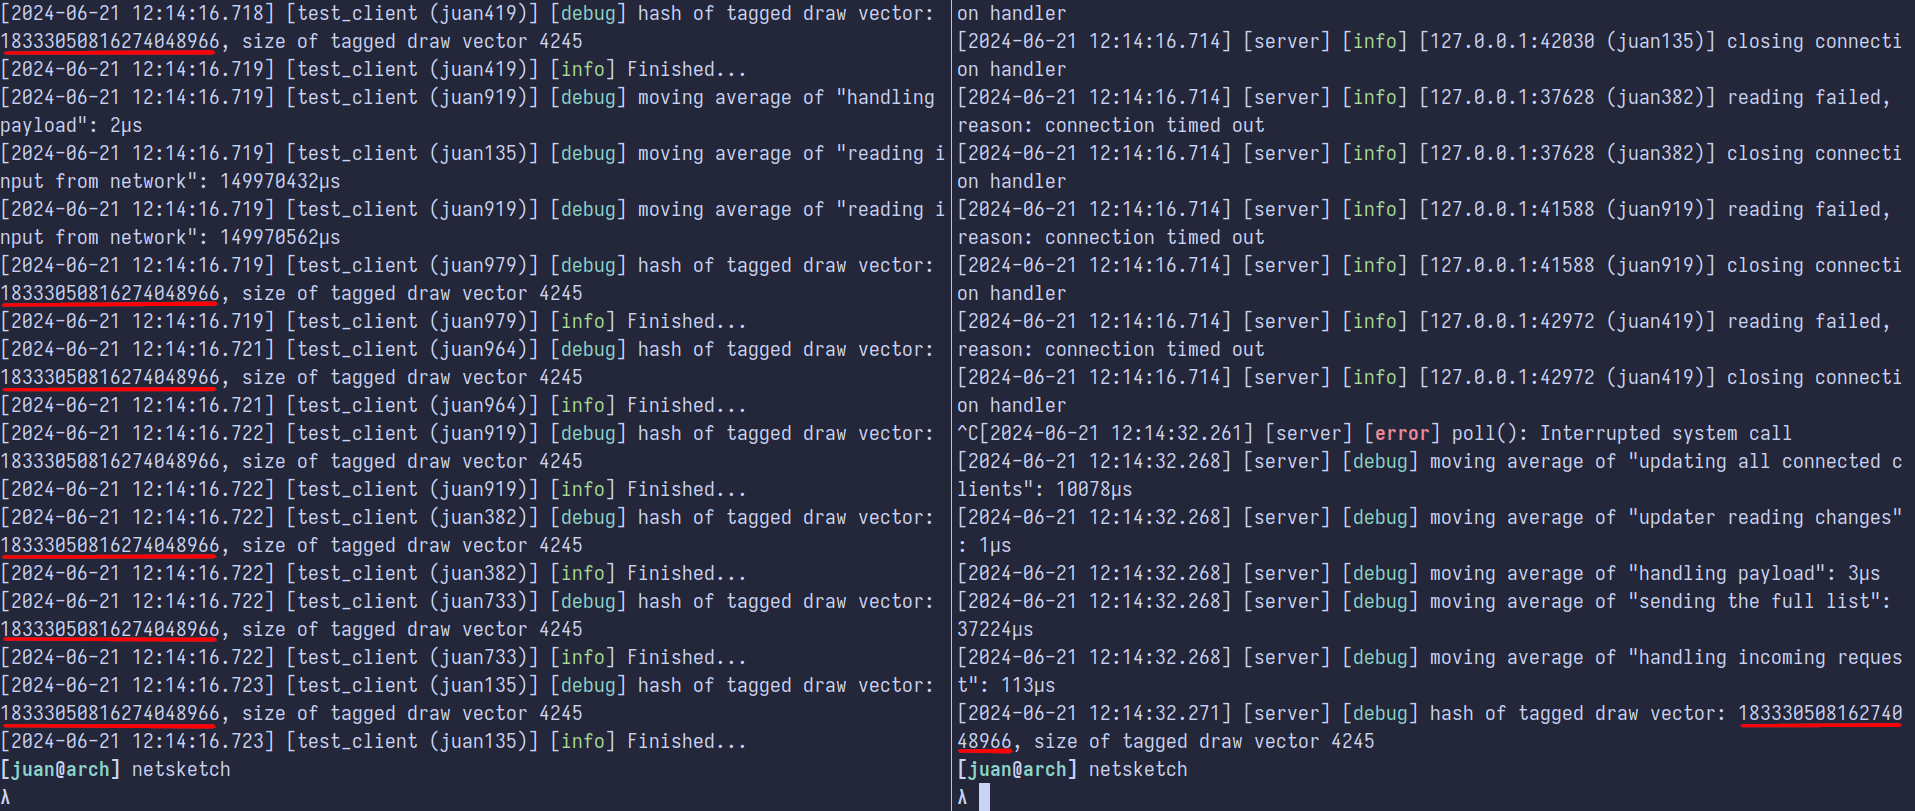
\includegraphics[width=\linewidth]{difficult-stress-other-end.png}
\caption{End phase of a stress test with 1000 test clients (with
other actions enabled and highlighted tagged draw vector
hashes).}
\label{fig:end1000stressother}
\end{figure}

Finally, a test with other actions for the test clients enabled
was conducted. A similar conlusion was reached. The server's
mechanisms for synchronisation appear to be robust (see Figure
\ref{fig:start1000stressother}, Figure
\ref{fig:timeout1000stressother} and Figure
\ref{fig:end1000stressother}).

\subsubsection{Testing Performance}

\begin{figure}[H]
\centering
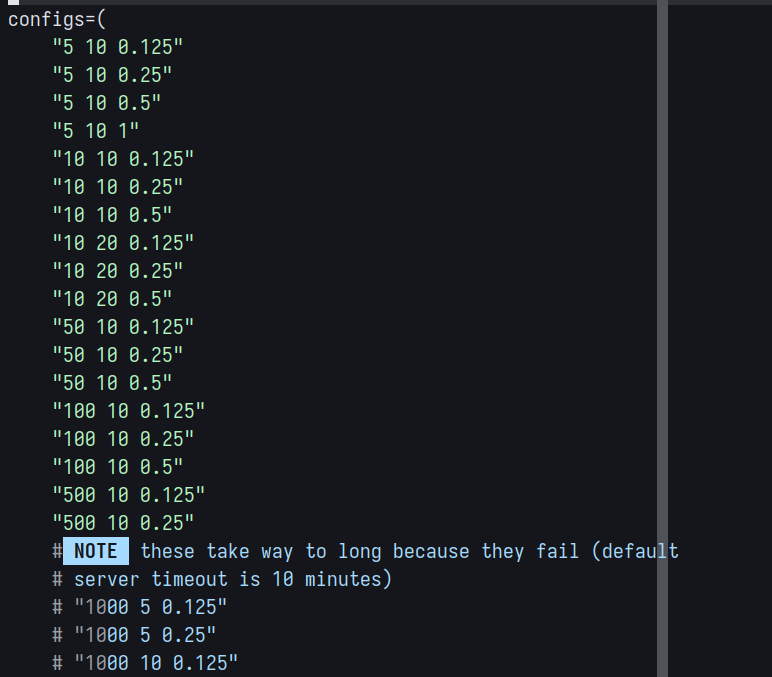
\includegraphics[width=\linewidth]{stress-configs.png}
\caption{All the different configurations used for testing and
data collection (each string  ``c i t'' is understood as the
number of clients (= `c'), the number of iterations (= `i') and
the time interval between each iteration (= `t').}
\label{fig:stressconfigs}
\end{figure}

When testing for performance the \texttt{collect-data.sh} script
was used. In particular, it contains a selection of
configurations (see Figure \ref{fig:stressconfigs}) for which it
is known that all the simultaneously generated connections can
be handled.

\begin{marker}
    Such a claim only hold on the machine which the project
    was developed on.
\end{marker}

\begin{figure}[H]
\centering
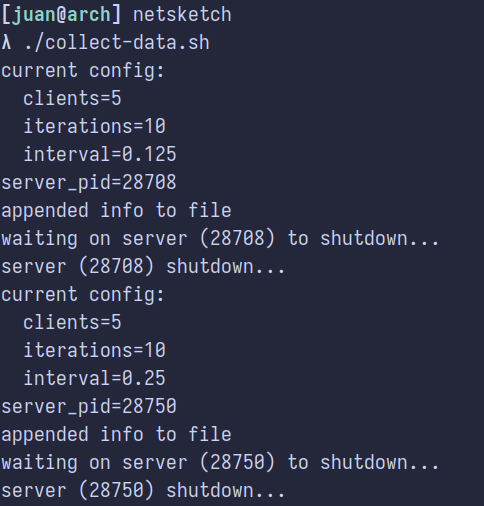
\includegraphics[width=\linewidth]{running-collect-data.png}
\caption{An example of the \texttt{collect-data.sh} script
running.}
\label{fig:runningcollectdata}
\end{figure}

\begin{marker}
    The script \texttt{collect-data.sh} connects to any
    currently running server. If none exist it will manage
    starting and shutting down instances itself (as it does in
    Figure \ref{fig:runningcollectdata}).
\end{marker}

\begin{figure}[H]
\centering
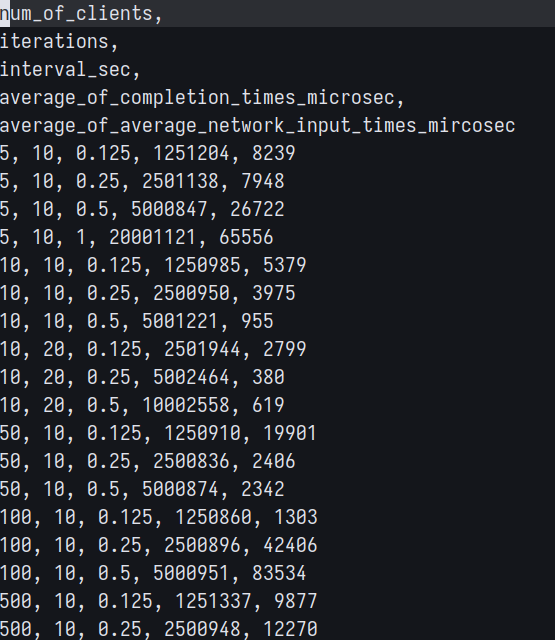
\includegraphics[width=\linewidth]{collected-data.png}
\caption{The collected data from running
\texttt{collect-data.sh} in the produces \texttt{data.csv}
file.}
\label{fig:collecteddata}
\end{figure}

\begin{figure}[H]
\centering
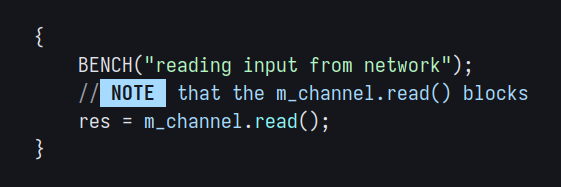
\includegraphics[width=\linewidth]{readingfromnetwork}
\caption{The \texttt{"reading input from network"} benchmark in
\texttt{src/test\_client/reader.cpp} at line 45.}
\label{fig:readingfromnetwork}
\end{figure}

In particular, looking at the outcome of the script (see Figure
\ref{fig:collecteddata}), the time it takes for each test client
in the scope of a specific configuration is very much linked to
the specified interval and the number of iterations.

In fact, if for each configuration the calculation
$\mathtt{iterations} * \mathtt{interval\_sec} * 1000000$ is
performed it is roughly equal to the completion time for each
test client (in the context of that configuration).

The average amount of time it takes to read a response is quite
inconsistent across the board. It seems to be really dependent
on the load of current machine hosting the server. However,
there does seem a slight up tick for longer intervals.

From the above observations one can conclude the following:

{\em
The amount of time it takes for a client (call it $C$) to
terminate is equivalent to the amount of time it would take for
all the clients (including $C$) to send all the draw commands
sequentially, to $C$.
}

This is indeed what was warned in Subsection
\ref{subsec:updatermodel}. The responsiveness of the application
is indeed dependent on the single-threaded performance of the
server. However, the amount of time the server spends doing
`other things', outside of the ideal scenario (where the time
would be exactly that computed using the above formula), is
minimal. Hence, this indicates a overall reasonable performance.

\begin{marker}
    One has to keep in mind that all these test were performed
    locally, where the performance penalty imposed by network
    congestion is close to zero.
\end{marker}

\subsection{Running \texttt{valgrind} on the Server}

\begin{figure}[H]
\centering
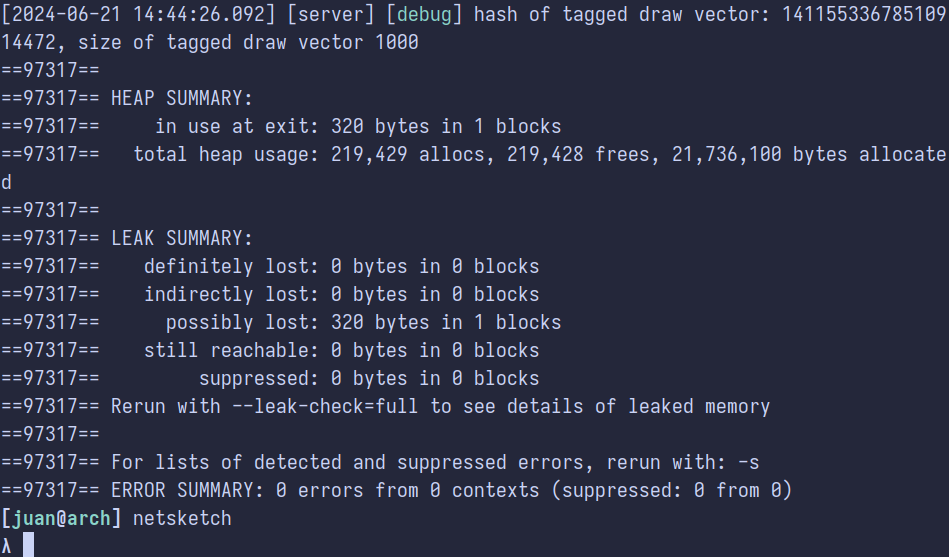
\includegraphics[width=\linewidth]{valgrind-test}
\caption{The result of running \texttt{./stress-server 100 10
0.25} with the server being instrumented with
\texttt{valgrind} (the single lost allocation has
been clarified in Section \ref{sec:posixwrappers}).}
\label{fig:valgrindservertest}
\end{figure}

Finally, the server was tested with \texttt{valgrind} to ensure
that over time the server does not consume more and more memory,
which could lead to the system failing (see Figure
\ref{fig:valgrindservertest}).

\subsection{Testing the Client}

\subsubsection{Performance Testing}

To test the actual client, CLion was used. CLion provides
facilities for generating flamegraphs and the client was tested
using these facilities.

\begin{attrib}
    The clear summary about flamegraphs provided by Brendan
    Gregg on his website
    \url{https://www.brendangregg.com/flamegraphs.html} was
    consulted.
\end{attrib}

\begin{figure}[H]
\centering
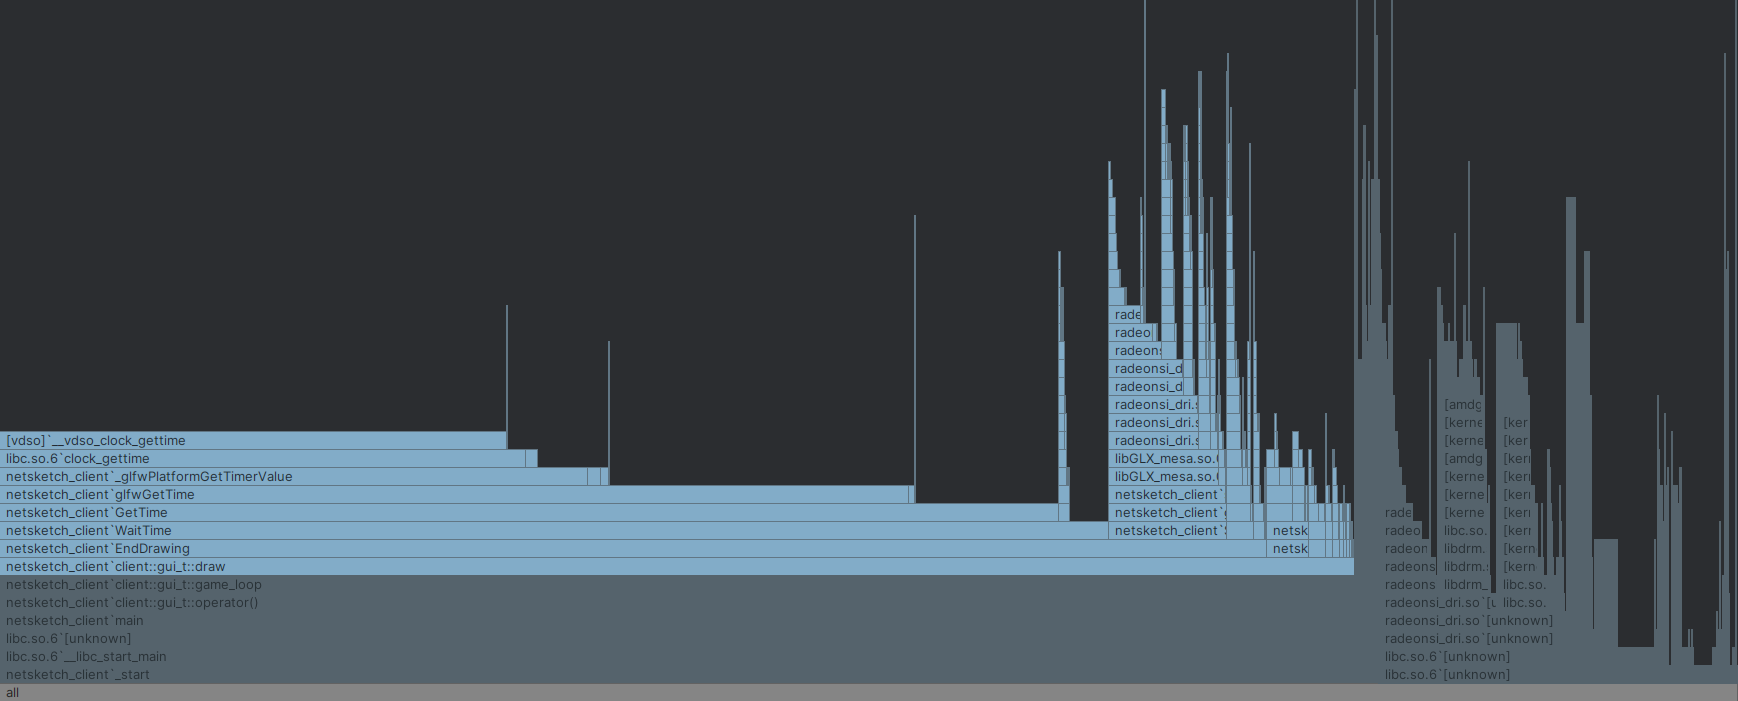
\includegraphics[width=\linewidth]{flamegraph1}
\caption{A flamegraph of the client running captured by CLion.}
\label{fig:flamegraph}
\end{figure}

\begin{figure}[H]
\centering
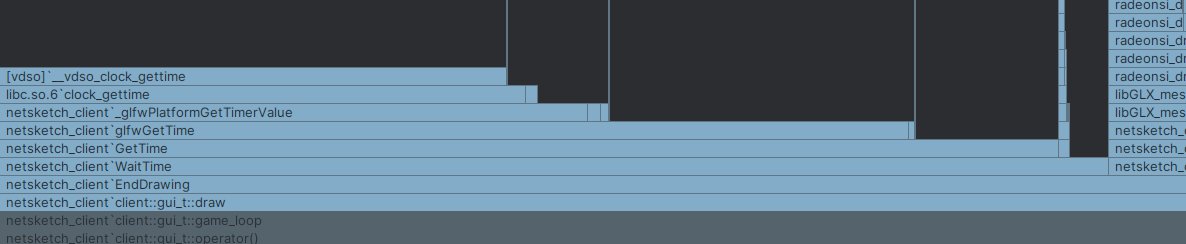
\includegraphics[width=\linewidth]{flamegraph1zoomed}
\caption{The same flamegraph as Figure \ref{fig:flamegraph} but zoomed (for clarity).}
\label{fig:flamegraphzoomed}
\end{figure}

As can be seen from Figure \ref{fig:flamegraphzoomed}, the
hottest path i.e. the path which has the most calls is the draw
function in the client. This means that the largest bottle neck
in the client is actually the drawing.

\begin{figure}[H]
\centering
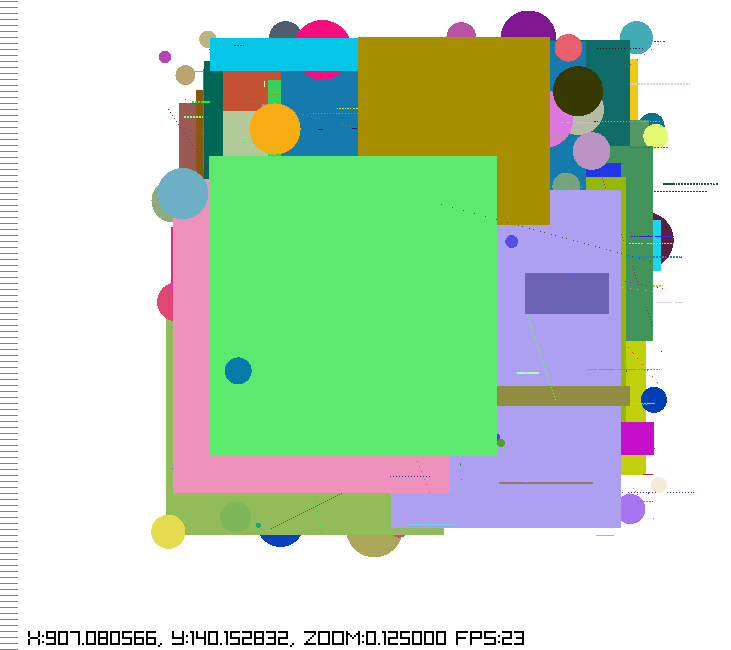
\includegraphics[width=\linewidth]{morethan5000fps}
\caption{A screenshot of a single client connected to the server
with many draw calls (notice that the FPS counter is sitting at
around 23).}
\label{fig:stressedclient}
\end{figure}

\begin{figure}[H]
\centering
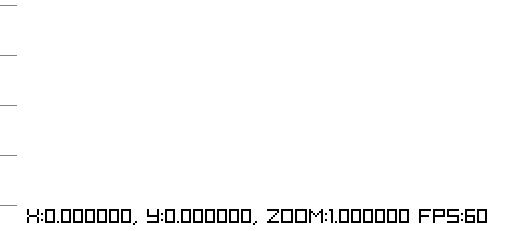
\includegraphics[width=\linewidth]{freshserverfps}
\caption{A screenshot of a single client connected to a fresh
server (notice that the FPS counter is sitting at around 60,
which is the cap imposed because of VSYNC).}
\label{fig:freshclient}
\end{figure}

This is corroborated by the result of running the
\texttt{collect-data.sh} script three times on an already open
server (see Figure \ref{fig:stressedclient} and Figure
\ref{fig:freshclient}). It is clear that the FPS has dropped
significantly. To solve this issue further work on the
representation of the drawings is required along with possible
improvements to the actual rendering it self. However, for such
changes direct modifications to Raylib or a different rendering
engine needs to be used.

\subsubsection{Input Testing}

\begin{figure}[H]
\centering
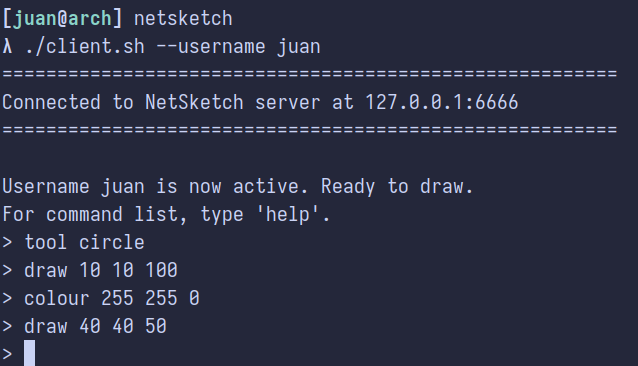
\includegraphics[width=\linewidth]{basic-input-example}
\caption{A screenshot of some basic input into a client.}
\end{figure}

A very rudimentary approach to testing the input mechanism was
used. In particular, the command line interface was manually
tested to ensure that at its most basic the inputs were properly
parsed.

\section{Recording}

For a more thorough walk-through of how the interface can be
used and how the clients and the server behave please have a
look at the video presentation which is being hosted at
\url{https://drive.google.com/file/d/1VMXR4Z0s5iDvXcroMTLn6ddb5enplOTF/view?usp=drive_link}.

\section{\textbf{Bonus}: The Exporter}

\begin{figure}[H]
\centering
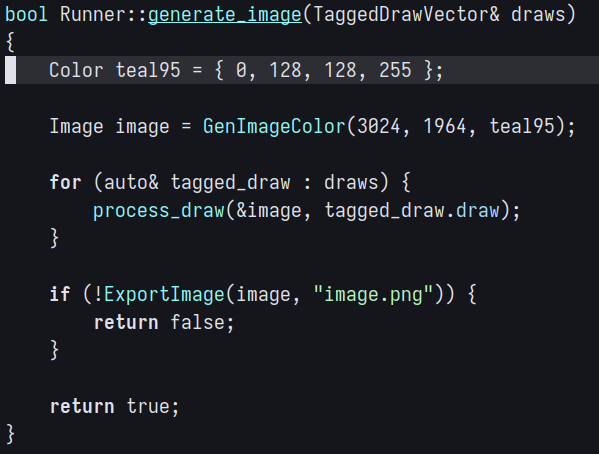
\includegraphics[width=\linewidth]{generate-image}
\caption{A screenshot of the generate image method in
\texttt{src/exporter/runner.cpp} at line 244.}
\end{figure}

The exporter is a simple binary which connects to an already
running server. It then uses Raylib's built in software renderer
to generate an image of the server's local tagged draw vector
with a specific background colour.

Of course, later on this can be directly embedded into the
client, using the GPU buffer instead of software rendering. But
for now it is sufficient for some cool backgrounds.

\begin{figure}[H]
\centering

\includegraphics[width=\linewidth]{exported-background}
\caption{A cool background generated by using the exporter.}
\end{figure}

\end{document}
